\documentclass{article}
\usepackage[margin=1in]{geometry}
\usepackage{array}
\usepackage{graphicx}
\usepackage{natbib}
\usepackage{amsmath, amssymb}
\usepackage{caption}
\usepackage[title]{appendix}
\usepackage[ruled]{algorithm2e}

\author{Carl Ehrett, Andrew Brown, Evan Chodora, \\Mingzhe Jiang, Christopher Kitchens, Sez Atamturktur}
%\date{}
\title{Computer model calibration as a method of design}

\begin{document}

\maketitle

\begin{abstract}
A well-established framework for the calibration of computer models is provided by \cite{Kennedy2001} and the myriad works that build upon it. 
%
Common to those approaches is the assumption that calibration is a matter of estimating unknown and/or uncontrollable parameters by attuning the model to data obtained through physical experimentation. 
%
In this work we reconceptualize model calibration as a method for optimization. 
%
Rather than calibrating a model to find a posterior distribution of unknown parameters in order to bring the model as much into agreement with reality as possible, we calibrate to find a posterior distribution on controllable model inputs in order to bring the predicted system behavior into agreement with pre-determined performance targets. 
%
In essence, we treat performance targets as ``desired observations'' and use them as the data in the calibration problem. 
%
We demonstrate our proposed methodology in both an artificial case and in the case of a finite element model of wind turbine blade performance and cost. 
%
In the latter case, we demonstrate how to estimate the Pareto front with uncertainty bands.\\

{{\bf Keywords:} Uncertainty quantification, Gaussian processes, optimization, Pareto optimality, wind turbines, material design}
\end{abstract}

\section{Introduction} \label{introduction}
% Discussion of computer experiments and computer model calibration. Lit review. Overview of project goals.

%\subsection{Computer experiments} \label{computer_experiments}

%Suppose that one wishes to improve one's understanding of, say, the movement of people in a crowd escaping from a building in a crisis situation. This is an example of an area in which field data, i.e.\ real-world observations, are extremely difficult to acquire. Merely assembling a crowd of research subjects in one place is costly and difficult. Asking them to flee a building may result in behaviors which are unlike those in real crisis situations -- but which may nonetheless present unacceptable physical risk to the subjects. Inducing them to flee through the generation of a (real or apparent) crisis is similarly infeasible. Observational data are likewise scarce here, since panic-inducing crises are by their nature difficult to predict and chaotic in ways that hinder the orderly collection of data.

%In the face of these difficulties, computer models offer a third alternative to the choice between attempting field data collection and giving up on the hope of progress. Using existing theory concerning human psychology and movement, it is possible to construct a computer model simulating the behavior of people evacuating from a large building. For example, the SIMULEX model described by \cite{Thompson1995} allows one to observe simulated evacuation behaviors.
%The user provides as input floor plans for each floor of the building (via CAD-based .dxf files), the locations of staircases and exits, the locations of occupants, the dimensions of their bodies, routes to exits, and a distribution on the response time of each occupant. 
% in any specified building layout, using any desired physical distribution of individuals, whose individual relevant characteristics (walking speed, initial body orientation, etc) may be controlled by the researcher. 
%The user can then observe how long it takes each occupant to exit the building.
%Thus, computer models provide a means to collect data which might otherwise be largely inaccessible. 

%The study of computer models from a statistical perspective calls for specialized tools and techniques. Gaussian processes (GPs) are popular for modeling the output of computer code when the code is too computationally expensive to allow for repeated evaluation. The GP then provides a computationally inexpensive emulator for the computer code. There are three reasons the popularity of GPs as emulators: (1) The use of a GP does not require detailed foreknowledge of the approximate parametric form of the computer model. Researchers often lack such foreknowledge in the case of complex computer models. (2) GPs easily interpolate the observed data. This is an advantage when the observations come from deterministic computer code that is free of observation error. (3) The variance of a GP provides a natural form of uncertainty quantification. 
%A Bayesian approach to the study of computer models is undertaken by \cite{Currin1991}; the authors approach GPs as prior distributions on the unknown form of the computer model. A frequentist application of GPs to computer models is provided by \cite{Sacks1989}, who use GPs not only for estimating uncertainty but also as the basis for their approach to experimental design in the area of deterministic computer models.  \cite{Santner2003a} offer a comprehensive discussion of the use of GPs for prediction, design, and sensitivity analysis with respect to computer experiments from both frequentist and Bayesian perspectives. It is against the background of these works that the past two decades of research into computer model calibration takes place.
%
%\subsection{Computer model calibration} \label{computer_model_calibration}
%
%Suppose that we wish to use the SIMULEX model to compare two different proposed building codes to be enforced in a given area. We may use average body dimensions and average interpersonal distance as input parameters for this model, both to settle the initial physical distribution of people throughout the building and to influence their behavior during evacuation. It is well-established that average body dimensions \citep{Subramanian2011,Cavelaars2000} %\citep{Bornstein1976} 
%and interpersonal distance \citep{Sorokowska2017} vary across locales. These values may be unknown for the case of a particular region. Thus we may wish to find the true values for average body dimensions and interpersonal distance in that region. We may wish, in other words, to \textit{calibrate} these parameters in the model.

Broadly, in model calibration, one may consider a model to be of the form $\eta(\mathbf x,\boldsymbol \theta)$, where $(\mathbf x,\boldsymbol \theta)$ comprise all inputs to the model. 
%
Input vector $\mathbf x$ is the collection of inputs that are known and/or under the control of the researcher.
% (in the evacuation example, this would include the building layout).  
%
The vector of calibration inputs $\boldsymbol \theta$ is the collection of parameters the values of which are unknown. 
%
These must be estimated for successful simulation. 
%
Thus where $f$ describes the true system and $y$ an observation of that system, consider the model to be 
%
\begin{equation} \label{eq:model_gen}
y(\mathbf x)=f(\mathbf x)+\epsilon(\mathbf x)=\eta(\mathbf x,\boldsymbol \theta) + \delta(\mathbf x)+\epsilon(\mathbf x)
\end{equation} 
%
where $\delta(\cdot)$ describes the model discrepancy -- i.e., the bias of the model as an estimate of the real system -- and $\epsilon(\cdot)$ is a mean-zero observation error, often i.i.d.\ Gaussian. 
%
%Notice that we may write $f(x)=f(x,\theta)$ since $\theta$ does not vary in reality. 
%
To undertake model calibration, one must have access to at least some observations of the real system.%; it is to these real observations that we calibrate the computer model.

Much interest in the past two decades has centered on Bayesian methods for model calibration. 
%
The appeal of a Bayesian approach to model calibration is that the calibration parameters are a source of uncertainty for the model. 
%
This uncertainty should be quantified so that its effect on the model can be made explicit. 
%
One can thus use Bayesian methods to construct a posterior distribution of the calibration parameters which balances our prior knowledge about the calibration parameters with what can be learned from the available data, and which also allows for accurate uncertainty quantification on the model outputs. 

The work of \cite{Kennedy2001} offers a Bayesian approach to computer model calibration that allows for the uncertainty of the calibration parameters in the predictions of the resulting calibrated model.
% 
This area is furthered by \cite{Higdon2004}, who develop an approach that undertakes model calibration with quantification of the related uncertainty, as well as explicitly incorporating uncertainty regarding the computer model output, the bias of the computer model, and uncertainty due to observation error (of field data). 
%
Other contributions in this area come from \cite{Williams2006}, \cite{Bayarri}, \cite{Liu2009}, \cite{Bayarri2007}, \cite{Brynjarsdottir2014}, and \cite{Brown2016}.
%That approach is further refined and exemplified by \cite{Williams2006}.
%\cite{Loeppky2006} offer an MLE-based alternative to the Bayesian approach promulgated by Kennedy and O'Hagan, intending thereby to improve the identifiability of the calibration parameters in the face of model discrepancy. 
%\cite{Bayarri2007} extend the approach of Kennedy and O'Hagan, providing a framework that is intended to allow for simultaneous validation and calibration of a computer model (using the same training data). 
%Though they  work within the Bayesian framework set by Kennedy and O'Hagan, they show how a Bayesian analysis can be profitably attenuated through what they call ``modularization''. 
%Modularization refers to separating sources of information, so that the model has distinct components or ``modules'', rather than allowing all information to combine into a single analysis under the umbrella of Bayes' theorem. \cite{Liu2009} focus directly on the use of modularization, exploring its advantages and disadvantages; amongst other potential motivations, they show that modularization can improve the identifiability of calibration parameters. 
%\cite{Bayarri} further the work of \cite{Bayarri2007} by applying the latter's methodology to functional data. 
%To do so, the methodology for dealing with scalar data is hierarchically applied to the coefficients of a wavelet representation of the functional data. Similarly, \cite{Paulo2012} focus on applying the lessons of \cite{Bayarri2007} to computer models with multivariate output.

%Above, I have described model calibration as a matter of estimating the true values of unknown parameters. Indeed, that is the sort of model calibration that will form the focus of the present work. However, in a broad sense of the term, model calibration takes a second form as well. 

%For convenience, one may distinguish this second form by referring to it as \emph{tuning}, rather than as calibration. In model tuning, a computer model includes inputs which must be calibrated, but which have no particular interpretation; i.e., tuning parameters do not represent the truth regarding some value of the system being modeled. The work of \cite{Brynjarsdottir2014} emphasizes the distinction between calibration and tuning. They show that whereas a well-modeled discrepancy function ($\delta(\cdot)$ in (\ref{eq:model_gen})) may not be necessary for tuning, since the tuning process can accomplish much of the work of a discrepancy function, an accurate discrepancy function is crucial for calibration, for the same reason. Letting the calibration process take on the duties of the discrepancy function reduces the identifiability of the calibration parameters.
%
%Another extension of the framework of \cite{Kennedy2001} and \cite{Bayarri2007} is \emph{state-aware} calibration \citep{Atamturktur2015,Stevens2018,Brown2016}. When one knows or suspects that the appropriate value of a calibration parameter $\boldsymbol \theta$ is dependent upon the other inputs $x$, state-aware calibration allows for the calibration procedure to estimate $\boldsymbol \theta$ as $\boldsymbol \theta(\mathbf x)$. This may obviate the need for a discrepancy function, either because the true value of the calibration parameter does indeed vary with the other inputs, or (in a tuning problem) because varying the tuning parameter can accomplish the work of a discrepancy function in aligning the computer model response with reality.

Common to these approaches is the conception of calibration as a matter of aligning the computer model output to observations of the real system. 
%
In this paper, we explore the idea of calibrating a computer model to align with performance targets, in order to find system settings that optimize performance with respect to those targets.
%
In the remainder of Section \ref{introduction}, we describe the calibration framework which we go on in Section \ref{calib_for_design} to adapt as a method for optimization. 
%
In Sections \ref{example} and \ref{application} we apply the proposed methodology to an example involving simulated data, and to an application in which the goal is to find material design settings to optimize the performance of a wind turbine blade.
%
Section \ref{application} we also apply the methodology to produce an estimate of the entire Pareto front of the (trivariate) system, where the Pareto front is the set of inputs such that making any of the system outputs better off would require making one or more of the outputs worse off. 
%
Section \ref{conclusion} concludes with discussion of the results.

\subsection{Calibration framework} \label{calib_framework}

In describing the calibration framework we use in this work, we here assume the use of a Gaussian process (GP) emulator of the computer model.
%
In principle, model calibration
%\footnote{In this work, ``calibration'' will usually be used broadly to include model tuning; where it is used in such a way as to exclude tuning, this will be made clear in context.}
need not rely on a GP emulator, or any other sort of emulator; one could (e.g.) complete a full Bayesian analysis via an MCMC chain that involves running the relevant computer model at each iteration of the chain. 
%
Indeed, in Section \ref{example} we perform calibration on our example simulated data without an emulator.
%
However, computer models are frequently too computationally expensive to allow for such profligacy.
%
Instead, a computationally tractable emulator can be constructed using a sample of observations from the computer model. 
%
GPs are popular prior distributions on computer model output for three reasons.
%
Firstly, because their use does not require detailed foreknowledge of the model function's parametric form. 
%
Secondly, GPs easily interpolate the computer model output, which is attractive when the computer model is deterministic. 
%
This is usually the case, although some attention in model calibration has focused specifically on stochastic computer models; see e.g.\ \cite{Pratola2018}. 
%
Thirdly, GPs facilitate uncertainty quantification through the variance of the posterior GP. 
%
This section provides brief background on Gaussian processes and their use in regression broadly and in computer model calibration specifically.

%\paragraph{Background}

%Gaussian processes can be thought of as generalizations of multivariate normal distributions. Whereas a multivariate normal random variable is a random vector of finite length, a realization of a Gaussian process can be thought of as a random function. The value of the function at any finite selection of points is itself a multivariate normal random variable. Just as a multivariate Gaussian random variable is characterized by its mean vector and covariance matrix, a Gaussian process is fully characterized by its mean function $\mu:D\to \mathbb R$ and covariance function $C:D\times D\to \mathbb R$, where $D$ is the domain of the process. Thus for any points $\mathbf x,\mathbf y$ in the domain of the Gaussian process, $\mu(\mathbf x)$ gives the mean of the Gaussian process at $\mathbf x$, and $C(\mathbf x, \mathbf y)$ gives the covariance between the values of the Gaussian process at points $\mathbf x$ and $\mathbf y$. As a special case, then, $C(\mathbf x,\mathbf x)$ gives the marginal variance of the GP at $\mathbf x$. 
%
%%\paragraph{Gaussian process regression}
%
%\cite{OHagan1978} suggested the use of GPs as priors for modeling unknown functions. Given observations $\mathbf f$ from the function $f$ being modeled, an updated mean and covariance function $\mu^*(\mathbf x)=\mu(\mathbf x)|\mathbf f$ and $C^*(\mathbf x,\mathbf y) = C(\mathbf x,\mathbf y)|\mathbf f$ describe a new GP that has been ``trained'' on the observations $\mathbf f$. 
%%O'Hagan did not focus in that work on applications to computer models.
%Though the approach of \cite{OHagan1978} was Bayesian, it did not provide for Bayesian means of selecting a covariance function $C$. \cite{Neal} extends the work of O'Hagan in this direction. \cite{Savitsky2011} describes a method for variable selection in GP regression via spike-and-slab mixture priors on the parameters of the covariance function. \cite{Shang2013} provide an umbrella generalization of existing methods of GP regression under a framework of what they call generalized GP models. \cite{Rasmussen2006} provide a comprehensive exploration of the use of GPs for regression and classification. All of these works treat GP regression generally, and do not focus specifically on the use of GPs to build emulators for computer models.

The use of GPs to produce a computationally efficient predictor $\hat \eta (\mathbf x)$ of expensive computer code $\eta(\mathbf x)$ given observations of code output at $\mathbf X=(\mathbf x_1,\ldots,\mathbf x_n)^T$ is promulgated by \cite{Sacks1989} and explored at length by \cite{Santner2003a}.
%
Since computer code is typically deterministic, these applications differ from the focus of \cite{OHagan1978} in that the updated GP is induced to interpolate the observations $\boldsymbol \eta = (\eta(\mathbf x_1),\cdots,\eta(\mathbf x_n))^T$. 
%
%Much recent attention in the wake of these efforts by Santner et al.\ and Sacks et al.\  has focused specifically on the use of GPs for computer model emulation.
%By contrast, much recent attention following the work of \cite{Santner2003a} and \cite{Sacks1989} has focused specifically on the use of GPs for computer model emulation. 
\cite{Kennedy2001} develop an influential framework for Bayesian analysis using GPs specifically for computer model calibration. 
%
\cite{Kennedy2006} showcase this use of GP emulators for uncertainty and sensitivity analyses. 
%
\cite{Bastos2009} describe both numerical and graphical diagnostic techniques for assessing when a GP emulator of a computer model is successful, as well as discussion of likely causes of poor diagnostic results. 
%
While most work in the area of GP emulation uses stationary covariance functions (in which $\mu(\cdot)$ is constant and $C(\mathbf x,\mathbf x' )\equiv C(\mathbf x-\mathbf x' )$ depends only on the difference between $\mathbf x$ and $\mathbf x'$, rather than on their location in the input domain) and quantitative inputs, efforts have been made to branch away from these core uses. 
%
\cite{Gramacy2008} use treed partitioning to deal with a nonstationary computer model. 
%
\cite{Qian2008} explore methods for using GP emulators that include both quantitative and qualitative inputs.

%As in any instance of GP regression, ``training'' a GP as a computer model emulator involves finding an updated mean and covariance function given a set of observations. The updated mean allows for prediction of the computer model at points not observed, with uncertainty quantified by the updated covariance function.
%Suppose, for example, that we begin with a prior GP with constant mean function $\mu(\mathbf x)=0$ for all $\mathbf x$. Notice that we may use the covariance function $C$ to define an $n\times n$ matrix $\mathbf C_{\mathbf X,\mathbf X}$ such that the $i,j$ entry of $\mathbf C_{\mathbf X,\mathbf X}$ is equal to $C(\mathbf x_i,\mathbf x_j)$. We may wish to train our GP on these $n$ observations, and then examine the resulting posterior GP given the points $\mathbf X'=(\mathbf x_1',\ldots,\mathbf x_m')^T$. Recall that the GP at the points $\mathbf X'$ is a multivariate normal random variable of length $m$, which is fully characterized by its mean vector $\mu^*_{\mathbf X'}$ and covariance matrix $\mathbf C^*_{\mathbf X',\mathbf X'}$. We can find these as:
%\begin{equation}\label{eq:post_gp}\begin{split}
%\mu^*_{\mathbf X'}&=\mathbf C_{\mathbf X',\mathbf X}\cdot \mathbf C_{\mathbf X,\mathbf X} ^{-1}\cdot \boldsymbol \eta
%\\
%\mathbf C^*_{\mathbf X'}&=\mathbf C_{\mathbf X',\mathbf X'}-\mathbf C_{\mathbf X',\mathbf X}\cdot \mathbf C_{\mathbf X,\mathbf X}^{-1}\cdot \mathbf C_{\mathbf X,\mathbf X'}
%\end{split}\end{equation}
%A visualization of this example is displayed in Figure \ref{fig:gp_example}. Here, $n=5$, and $x'=(-5,-4.75,\ldots,4.75,5)$. 

%\begin{figure}[h]
%\centering
%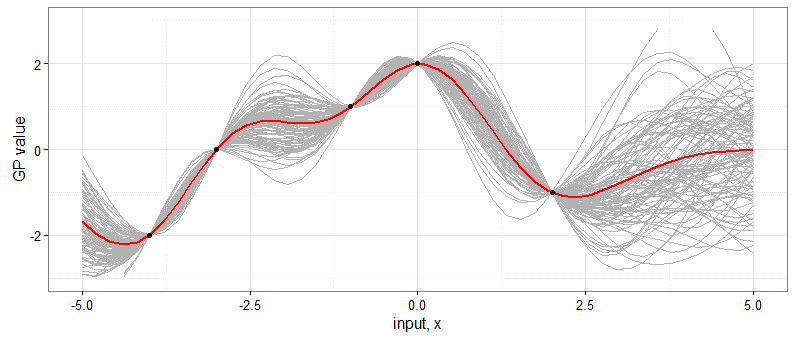
\includegraphics[width=.75\linewidth]{gp_example}
%\captionsetup{width=.7\linewidth}
%\caption{Example of a Gaussian process trained to interpolate five data points (black dots). The posterior mean function is shown in red; the gray lines are 50 draws from the posterior GP.}
%\label{fig:gp_example}
%\end{figure}

%\paragraph{Gaussian processes in computer model calibration}

%Aside from \cite{Kennedy2001}, recent applications of GP emulation specifically to problems of calibration have focused largely on the works of \cite{Williams2006} and \cite{Bayarri2007}. 
%%
%It is helpful here to provide an illustrative summary of the approach taken by \cite{Williams2006}, both to exemplify the use of GPs for computer model calibration and because the approach utilized in the present work closely follows theirs.

Suppose that we have inputs $\{\mathbf x_i\}_{i=1}^n\subseteq \mathbb R^p$ scaled to the unit hypercube, and observations 
%
\begin{equation}\label{eq:2}
y(\mathbf x_i) = f(\mathbf x_i) + \epsilon(\mathbf x_i),\quad i=1,\cdots,n,
\end{equation}
%
where $f(\cdot)$ is the true system and $\epsilon(\cdot)$ is known measurement error. 
%
Then by \eqref{eq:model_gen} we have
%
\begin{equation}\label{eq:2}
y(\mathbf x_i) = \eta(\mathbf x_i,\boldsymbol \theta) + \delta(\mathbf x_i) + \epsilon(\mathbf x_i),\quad i=1,\cdots,n
\end{equation}
%
where $\eta(\cdot,\cdot)$ is the computer model, $\boldsymbol \theta$ is the best%\footnote{In the case of calibration, the ``best'' setting will be the true setting of that parameter; in a case of tuning rather than calibration, the ``best'' setting would instead be the optimal setting for minimizing model bias.}
setting of the vector of calibration parameters, and $\delta(\cdot)$ is the discrepancy function describing the bias of $\eta(\cdot,\cdot)$ as an estimate of $f(\cdot)$.
\citeauthor*{Williams2006} define the GP prior for modeling $\eta(\cdot,\cdot)$ as follows. 
%
Let the mean function $\mu(\mathbf x,\mathbf t)=c$, $c$ a constant. 
%
Set the covariance function in terms of the marginal precision $\lambda_\eta$ and a product power exponential correlation function:
%
\begin{equation}\label{eq:Hig_cov}
C((\mathbf x,\mathbf t),(\mathbf x',\mathbf t')) = \frac 1\lambda_\eta \prod_{k=1}^{p}
\exp \left(-\beta^\eta_k|x_k-x_k'|^{\alpha_\eta}\right) \times
\prod_{k=1}^{q}
\exp \left(-\beta^\eta_{p+k}|t_k-t_k'|^{\alpha_\eta}\right)
\end{equation}
%
where each $\beta_k$ describes the strength of the GP's dependence on one of the elements of the input vectors $\mathbf x,\mathbf t$, and $\alpha_\eta$ determines the smoothness of the GP. 

The authors place the following priors on the hyperparameters:
%
\begin{equation}
\begin{aligned}
c&\sim N(0,v)\\
\lambda_\eta&\sim \mathrm{Gamma}(5,5),\quad\lambda_\eta>0\\
\rho_k^\eta &\sim \mathrm{Beta}(1,0.1),\quad k=1,\cdots,p+q
\end{aligned}
\end{equation}
%
where $\rho_k^\eta=\exp(-\beta_k^\eta/4)$ for $k=1,\cdots,p+q$. 
%
They set $\alpha_\eta=2$, which corresponds to the assumption of an infinitely differentiable correlation function. 
%
The parameters of the Gamma and Beta distributions are chosen to encourage $\lambda_\eta$ to be close to one, and $\beta_k$ to be low for all $k$ (encouraging strong dependence; i.e., we antecedently expect each of the inputs to be influential). 
%
Furthermore, the authors let $v\to0$, i.e., the GP is assumed to have constant mean $c=0$.

The authors similarly model the discrepancy term as a GP, also with mean zero, and covariance function
%
\begin{equation}
C_\delta(\mathbf x,\mathbf x') = \frac 1{\lambda_\delta} \prod_{k=1}^p
\exp\left( -\beta_k^\delta |x_k-x_k'|^{\alpha_\delta} \right),
\end{equation}
%
with priors
%
\begin{equation}
\begin{aligned}
\lambda_\delta &\sim \mathrm{Gamma}(a_\delta,b_\delta)\\
\rho^\delta_k &\sim \mathrm{Beta}(1,0.3).
\end{aligned}
\end{equation}
%
where $\rho_k^\delta=\exp(-\beta_k^\delta/4)$ for $k=1,\ldots,p$ and $\alpha_\delta=2$.

Where $\boldsymbol \eta = (\eta(\mathbf x_1,\mathbf t_1),\cdots,\eta(\mathbf x_n,\mathbf t_n))^T$ are the simulation observations, $\mathbf y = (y(\mathbf x_{n+1}),\cdots,y(\mathbf x_{n+m}))^T\equiv (y(\mathbf x_{n+1},\boldsymbol\theta),\cdots,y(\mathbf x_{n+m},\boldsymbol\theta))^T$ are the field observations, $\mathcal D = (\boldsymbol \eta^T,\mathbf y^T)^T$, $\boldsymbol \beta^\eta = (\beta^\eta_1,\cdots,\beta_{p+q}^\eta)^T$, and $\boldsymbol \beta^\delta = (\beta^\delta_1,\cdots,\beta_{p+q}^\delta)^T$, we then have the distribution of $\mathcal D$ as 
%
\begin{equation}
\mathcal D | \boldsymbol \theta,c,\lambda_\eta, \boldsymbol \beta^\eta,\lambda_\delta,\boldsymbol \beta^\delta,\mathbf C_{\mathbf y} \sim N(c \cdot \mathbf 1_{n+m}, \mathbf C_{\mathcal D})
\end{equation}
%
where $\mathbf C_{\mathbf y}$ an $m\times m$ matrix in which the $i,j$ entry is the (known) observation variance $C_{obs}(\mathbf x_i,\mathbf x_j)$ for $n<i,j\leq n+m$, and $\mathbf C_{\mathcal D}$ is a matrix with its $i,j$ entry equal to
%
\begin{equation}\label{eq:C_D}
C((\mathbf x_i,\mathbf t_i),(\mathbf x_j,\mathbf t_j)) + I(i,j>n)\cdot(C_{obs}(\mathbf x_i,\mathbf x_j) + C_\delta(\mathbf x_i,\mathbf x_j))
\end{equation}

Thus, the joint posterior density under the model is
%
\begin{equation} \label{eq:full_dist}
\pi(\boldsymbol \theta,c,\lambda_\eta,\boldsymbol \rho^\eta,\lambda_\delta,\boldsymbol \rho^\delta,\mathbf C_{\mathbf y}|\mathcal D)
\propto \pi(\mathcal D | \boldsymbol \theta,c,\lambda_\eta, \boldsymbol \beta^\eta,\lambda_\delta,\boldsymbol \beta^\delta,\mathbf C_{\mathbf y}) \times \pi(c) \times \pi(\lambda_\eta) \times 
\pi(\boldsymbol \rho^\eta) \times \pi(\lambda_\delta) \times \pi(\boldsymbol \rho^\delta)
\end{equation}
%
Note that where a discrepancy function is not included in the model and the mean $c$ is treated as a constant, (\ref{eq:full_dist}) simplifies greatly; where furthermore $\lambda_\eta$ and $\boldsymbol \rho^\eta$ are estimated via maximum likelihood (as in  \cite{Kennedy2001}),  (\ref{eq:full_dist}) simplifies down merely to 
%
$\pi(\mathcal D | \boldsymbol \theta,c,\lambda_\eta, \boldsymbol \beta^\eta,\lambda_\delta,\boldsymbol \beta^\delta,\mathbf C_{\mathbf y})$. 
%
Markov chain Monte Carlo methods are useful for evaluating (\ref{eq:full_dist}).
%The next section takes up this topic.

%\subsubsection{Markov chain Monte Carlo methods}\label{MCMC_methods}
%
%%\paragraph{Background}
%
%The central idea of Markov chain Monte Carlo (MCMC) integration is to construct a Markov chain which has as its equilibrium distribution the target distribution one wishes to explore. The Markov chain is observed, and beyond an initial ``burn-in'' period during which the chain is allowed to approach its equilibrium distribution, samples are considered to be drawn approximately from the target distribution.
%
%For example, consider a model with posterior distribution given by (\ref{eq:full_dist}), but where discrepancy is not included and $\lambda_\eta,\boldsymbol \rho^\eta$ are found via maximum likelihood estimation. Then the full distribution is given by $\pi(\boldsymbol \theta,c,\lambda_\eta,\boldsymbol \rho^\eta,\lambda_\delta,\boldsymbol \rho^\delta|\mathcal D)
%\propto \pi(\mathcal D | \boldsymbol \theta,c,\lambda_\eta, \boldsymbol \beta^\eta,\lambda_\delta,\boldsymbol \beta^\delta,\mathbf C_{\mathbf y}) \times \pi(c)$. A simple means of exploring this distribution via MCMC would begin with an initial guess $\boldsymbol \theta^{(1)},c^{(1)}$. At the $i^{\text{th} }$ step for $i=2,\ldots$, using a proposal distribution $q(\cdot,\cdot|{\boldsymbol\theta^{(i-1)},c^{(i-1)}})$ from which one may easily sample directly, one draws a new ``proposed'' sample $\boldsymbol \theta^*,c^*$. One then accepts this new proposed sample, setting $(\boldsymbol\theta^{(i)},c^{(i)}) = (\boldsymbol \theta^*,c^*)$, with probability
%\begin{equation}\label{eq:mh-acceptance}
%\alpha = \frac{\pi(\boldsymbol \theta^*,c^* | \mathcal D)}{ \pi(\boldsymbol \theta^{(i-1)},c^{(i-1)}|\mathcal D) } = 
%\frac{ \pi(\mathcal D | \boldsymbol \theta^*,c^*,\lambda_\eta, \boldsymbol \beta^\eta,\lambda_\delta,\boldsymbol \beta^\delta,\mathbf C_{\mathbf y}) \times \pi(c^*)}{\pi(\mathcal D | \boldsymbol \theta^{(i-1)},c^{(i-1)},\lambda_\eta, \boldsymbol \beta^\eta,\lambda_\delta,\boldsymbol \beta^\delta,\mathbf C_{\mathbf y}) \times \pi(c^{(i-1)})}.
%\end{equation}
%Otherwise one rejects the proposed sample and let $(\boldsymbol \theta^{(i)},c^{(i)}) = (\boldsymbol \theta^{(i-1)},c^{(i-1)})$. 
%In defining $\alpha$ in this way, it is assumed that $q$ is a symmetric distribution. The version of MCMC described in this example is known as the Metropolis algorithm. It was initially described by \cite{Metropolis1953}. \cite{Hastings1970} generalizes the technique (to what is now called the Metropolis-Hastings algorithm) so that it may utilize non-symmetric proposal distributions. A thorough exposition of the technique, its theoretical foundation, and its relation to other  varieties of MCMC is provided by \cite{Chib1995}.
%
%% Gibbs
%A related variant of MCMC -- in fact, a special case of Metropolis-Hastings, as shown by \cite{Gelman1992} -- is Gibbs sampling, initially described by \cite{Geman1984}. In using Gibbs sampling, one finds the conditional distribution of each of the parameters one wishes to sample, using the most recent samples of all other parameters. For example, we can convert the above Metropolis-Hastings illustration to a simple case of Gibbs sampling as follows.
%Begin as before, with initial guesses $\boldsymbol \theta^{(1)}$ and $c^{(1)}$. Thereafter, sample $\boldsymbol \theta$ and $c$ not together, but rather in alternating draws. That is, at the $i^{\text{th} }$ step for $i=2,\cdots$, draw $\boldsymbol \theta^{(i)}$ conditional on $c=c^{(i-1)}$, then draw $c^{(i)}$ conditional on $\boldsymbol \theta=\boldsymbol \theta^{(i)}$. Thus, for example, when drawing $c^{(i)}$, its conditional distribution would be proportional to $\pi(\mathcal D | \boldsymbol \theta^{(i)},c^{*},\lambda_\eta, \boldsymbol \beta^\eta,\lambda_\delta,\boldsymbol \beta^\delta,\mathbf C_{\mathbf y}) \times \pi(c^{*})$. 
%If the conditional distribution is something from which we may easily draw directly, then we can draw $c^{(i)}$ that way; otherwise, we can use a so-called Metropolis-within-Gibbs scheme, and draw $c^{(i)}$ similarly to what was described above for the Metropolis-Hastings algorithm: draw a proposed $c^*$ from a proposal distribution, find the appropriate ratio $\alpha_c$, and accept or reject $c^*$ accordingly. In the application considered in the present work, Metropolis-within-Gibbs is used.
%
%%\paragraph{Elimination of boundary constraints}
%
%Recall that a symmetric proposal distribution is required in order for the Metropolis algorithm to proceed as described in the above illustration of that technique. However, the algorithm can accommodate an asymmetric proposal distribution with only slight complication. One reason for using an asymmetric proposal distribution is as a means of accommodating boundary constraints on the parameter being sampled. Thus, for example, in the application considered in the present work, one of the calibration parameters is the thickness (in mm) of the material forming a wind turbine blade. Expert opinion was used to set the support of this parameter to be the range [10mm, 25mm]. Efficient exploration of the parameter space in the MCMC chain is promoted by choosing a proposal density such that the distribution $q(\cdot|\tau)$ has mean $\tau$. An asymmetric distribution can be used to accommodate the boundary constraints. When $q(\cdot|\tau)$ is asymmetric, this changes the above illustration only by way of requiring us to calculate the acceptance probability $\alpha$ as follows:
%\begin{equation}\label{eq:mh_correction}
%\alpha = \frac{\pi(\boldsymbol \theta^*,c^* | \mathcal D)}
%{ \pi(\boldsymbol \theta^{(i-1)},c^{(i-1)}|\mathcal D) } \times 
%\frac{
%q(\boldsymbol \theta^{(i-1)},c^{(i-1)}|\boldsymbol \theta^*,c^*)
%}{
%q(\boldsymbol \theta^*,c^*|\boldsymbol \theta^{(i-1)},c^{(i-1)})
%}.
%\end{equation}

%\subsubsection{Normalization of inputs and standardization of outputs}
%Blah

\subsubsection{Computational difficulties}
Consider a GP with constant mean function $\mu(\mathbf x)=0$ for all $\mathbf x$. 
%
We use the covariance function $C$ to define an $n\times n$ matrix $\mathbf C_{\mathbf X,\mathbf X}$ such that the $i,j$ entry of $\mathbf C_{\mathbf X,\mathbf X}$ is equal to $C(\mathbf x_i,\mathbf x_j)$. 
%
Training the GP on the $n$ observations $\boldsymbol \eta$ at $\mathbf X\in \mathbb R^{n\times p}$, an updated mean and covariance matrix for the points $\mathbf X'=(\mathbf x_1',\ldots,\mathbf x_m')^T$ is 
%. Recall that the GP at the points $\mathbf X'$ is a multivariate normal random variable of length $m$, which is fully characterized by its mean vector $\mu^*_{\mathbf X'}$ and covariance matrix $\mathbf C^*_{\mathbf X',\mathbf X'}$. We can find these as:
%
\begin{equation}\label{eq:post_gp}\begin{split}
\boldsymbol\mu^*_{\mathbf X'}&=\mathbf C_{\mathbf X',\mathbf X}\cdot \mathbf C_{\mathbf X,\mathbf X} ^{-1}\cdot \boldsymbol \eta
\\
\mathbf C^*_{\mathbf X'}&=\mathbf C_{\mathbf X',\mathbf X'}-\mathbf C_{\mathbf X',\mathbf X}\cdot \mathbf C_{\mathbf X,\mathbf X}^{-1}\cdot \mathbf C_{\mathbf X,\mathbf X'}
\end{split}\end{equation}
%
%Note that the joint posterior density given in (\ref{eq:full_dist}) above includes $\mathbf C_{\mathcal D}$, which, depending on how many field and simulation observations one has, may be of prohibitively high dimension. This can lead to computational difficulties in calculating $\alpha$ in the course of the MCMC routine. Difficulties arise in two ways. Firstly, the likelihood given in (\ref{eq:full_dist}) evaluated at a given point can be so small as to be vulnerable to significant round-off error. 
%
Poor conditioning of $\mathbf C_{\mathbf X,\mathbf X}$ in (\ref{eq:post_gp}) can make it difficult to invert and find the determinant of this matrix, as must be done in the course of the MCMC to find the relevant likelihoods.
%
This problem can be alleviated by adding a small nugget to $\mathbf C_{\mathbf X,\mathbf X}$. 
%
That is, we can set $\mathbf C_{\mathbf X,\mathbf X}^\xi= \mathbf C_{\mathbf X,\mathbf X} + \xi \cdot \mathbf I_{\mathrm{dim}(\mathbf X)}$ for some very small value of $\xi$, e.g., $\xi=10^{-4}$. 
%
Such a simple nugget works quite well in many applications. For a more sophisticated approach to selecting the nugget size, however, see \cite{Ranjan2011}. 
%
Note that adding a nugget here is equivalent to adding a small amount of observation variance for the simulator observations. 
%
That is, in adding this nugget, one no longer requires that the GP emulator precisely interpolate the simulation observations. 
%
However, for very small nuggets, this effect is so small as to be negligible, though the computational benefits remain. 
%
%Thus nothing is lost in continuing to think of the GP emulator as interpolating the simulation observations.
%
Furthermore, insofar as the effect is non-negligible, it is argued by \cite{Gramacy2012} to be beneficial for emulating the computer code (so that for some applications one might prefer a larger nugget).

%The other problem -- round-off error due to small likelihoods -- can be alleviated through substituting the use of log-likelihoods in the MCMC routine. Thus, rather than finding $\alpha$ in \eqref{eq:mh_correction} directly, it is preferable to find 
%\begin{equation}\label{eq:log_lik_alpha}
%\log \alpha = \log \pi(\boldsymbol \theta^*\!,c^* | \mathcal D) + \log q(\boldsymbol \theta^{(i-1)}\!,c^{(i-1)}|\boldsymbol \theta^*\!,c^*) - \log \pi(\boldsymbol \theta^{(i-1)}\!,c^{(i-1)}|\mathcal D) - \log q(\boldsymbol \theta^*\!,c^*|\boldsymbol \theta^{(i-1)}\!,c^{(i-1)})
%\end{equation}
%Of course, in order to enjoy the computational benefits of this approach, one must perform calculations on the log scale from the start; it would not do to, e.g., find $\pi(\boldsymbol \theta^*, c^*|\mathcal D)$ on its original scale and then take its log. 
% DISCUSS Better not to mention this?

\section{Calibration for design}\label{calib_for_design}

% Intro: description of sort of situation in which you'd want this

Suppose that a researcher has a fairly reliable computer model of a given system. 
%
Suppose furthermore that some of the parameters of that system can be controlled, and that the researcher hopes to select values for these controllable parameters that will facilitate certain target outcomes from the system. 
%
%An example would be selecting a building layout conducive to efficient evacuation, as modeled using SIMULEX.

%We may approach such problems as a matter of calibration. 
%
In traditional calibration as described in Section \ref{introduction}, a computer model is calibrated to physical observations. 
%
This is done in order to find settings for the computer model that induce its output to match reality as closely as possible. 
%
Similarly, one may seek to ``calibrate'' a computer model to a set of performance targets, in order to find settings that induce the model's output to match, or approximate, those targets. 
%
Hereafter, call performance targets treated as observations for the purpose of calibration ``desired observations''. 
%
Call the calibration procedure proposed here, which uses the model calibration framework of \cite{Kennedy2001} with desired observations, ``calibration to desired observations" (CDO). 

%Of course, computer models are more malleable than reality, and it is trivial to modify a computer model so that its output matches any given target. 
Computer models are more malleable than reality, and one might worry that in calibrating a model to unobserved performance targets, the model's fidelity to reality might be mitigated.
%
%It is both easy and pointless to create a model which is a computational ``yes man''. 
%
In many cases, however, one is fortunate to have (perhaps after undertaking traditional model calibration, validation and verification) a computer model such that one is confident that the model is known to be faithful to reality over a given set $\mathcal T$ of user specified calibration parameters.
%uniformly valid over a given set $\mathcal T$ of controllable parameters $t$, i.e., the model is known to be faithful to reality over $\mathcal T$. 
%
In such a circumstance, in calibrating $t\in\mathcal T$ to one's desires, one does not risk calibrating the model \emph{away} from agreement with reality, even if one's performance targets are not realistically achievable. 
%
Instead, one finds a distribution on the settings that achieve the best realistic approximation to the desired targets.

The tools of model calibration founded in the work of \cite{Kennedy2001} retain their advantages under the proposed application.
%
Most centrally, such calibration to desired observations $y$ produces not merely a static optimum $t\in\mathcal T$, but rather a posterior distribution of $t|y$ reflective of remaining uncertainty about the appropriate value of $t$. 
%
Such uncertainty may have its source in parameter uncertainty (uncertainty about the values of certain model inputs), code uncertainty (uncertainty about how closely the code approximates reality), and that which traditional calibration would consider observation error and model inadequacy. 
%
Of course,  targets are not actually observations, so the concept of observation error does not cleanly transfer. 
%
However, a similar uncertainty would be that due to how close reality \emph{can} come to our desired observations. 
% DISCUSS AB says explain this more. We have already discussed this a bit
%But just as the target can be treated as an observation in the calibration process, as it were \emph{aspirationally}, so too an observation error variance can be specified aspirationally, rather than as reflective of reality.
The model calibration framework of \cite{Kennedy2001} allows for the quantification of all of these uncertainties. Furthermore, by the use of informative priors on the model discrepancy and observation error, the identifiability concerns of the Kennedy-O'Hagan approach can be mitigated \citep{Bayarri2007,Tuo2016}.

\subsection{Target observations}
% This describes the basic idea.
% Include discussion: how do we select desired data?
% Also include discussion of how this is actually effected. This discussion will be short, because the answer is that it will use the framework described already in the previous section.


\subsubsection{Level of target data}\label{level_of_desired_data}
% Arbitrariness recommending prior on observation variance
Unlike in the case of field observations, when calibrating to performance targets treated as desired observations, the question arises of choosing what exactly those ``observations'' should be.
%
In many cases, no objectively natural target manifests itself. 
%
Indeed, there is no barrier to the use even of impossible targets such as negative values for model outputs known to be nonnegative.
%Consider, e.g., modeling the effect of building layouts on emergency evacuation time. 
%%
%In the case of a multi-story building, one might plausibly expect to achieve evacuation times of no less than fifteen minutes. 
%%
%But plausibility is no barrier to desire, and it would be a mistake to limit one's target observations to what is antecedently believed to be achievable, if only because to do so would foreclose on the possibility of exceeding those expectations. 
%%
%In the case of building evacuation, then, one might conclude that the appropriate target observation is in fact instantaneous evacuation -- \textit{per impossible}. 
%%
%But, having discarded realism, even this lower bound is not inevitable. Why not calibrate to a \emph{negative} evacuation time, while we're at it?
%
Such a target observation in certain situations may be appropriate. 
%
However, in general, target observations should aim only a little beyond what is realistically achievable; only as much as is necessary to ensure the targets are at least as ambitious as any true optimum in the system.
%
Three reasons why one should go only a little beyond that are as follows. 
%
(1) If target observations are set to be too farfetched, then the calibration can become computationally unstable due  to underflow and round-off error, since any value of $\boldsymbol \theta$ within its support will have extremely low likelihood.
% DISCUSS Andrew and I had talked about how this isn't quite true since the observation variance will expand to be as big as it needs to be to make the likelihoods work. But (a) some versions of CtDO call for a cap on observation variance / discrepancy variance, and (b) even with the version that lets obs var get as high as it likes, still there is a prior on obs var which penalizes high values of it, so it seems to me the point stands.
%
%
(2) Increasing the distance of the desired observations from the optimal region reduces the identifiability of that region.
%
The calibration finds the region of the parameter space with output closest to the target observations.
%
If the entire model range is far from the target observations, then the optimal region will in relative terms be only a little closer than the rest of the model range. 
% 
As a result, the identifiability of the optimal region will suffer.
%The nearness of the optimum to another point in the parameter space is relative to the estimated error at the optimum, and therefore if the entire model range is far from the target observations, then all points in the parameter space will be 
%
%relative difference between the distance to the Pareto front and the distance to other regions of the model range, thereby decreasing the identifiability of the region to which one wishes to calibrate.
%
(3) The desired observations lose a measure of interpretability when they delve too far into the fantastical, such as with impossibly negative values. 
%
Identifying the appropriate range of outputs for desired observations, which exceed reality only slightly, will often require one to consult a subject matter expert. 

%\subsubsection{Set target via desired observations, or prior distribution?}
%% DISCUSS (terminology of desired observations) % MAke clear that it is a term of art
%In undertaking model calibration to achieve desired system output, directly setting desired observations is not the only option. For example, in the application considered below in Section \ref{application}, the calibration parameters are controllable features of material design, and the cost of the resulting material is one of the outputs for which I establish targets. 
%%Two approaches are used for doing this. 
%One approach is simply to include a desired observation of cost, and calibrate to that along with the other desired observation targets. 
%An alternative approach is to remove cost from the model, and place a prior distribution on the remaining calibration parameters that places low probability over those regions of the calibration parameter space for which the cost is high. Of course, this requires prior knowledge of the behavior of cost over the calibration parameter space. Without such knowledge, this alternative would be unavailable.

A third option is also explored in Section \ref{application}'s treatment of the material design application. 
%
This option is not truly another means of achieving a calibration target, but rather is simply the decision to refrain from doing so. 
%
That is, rather than include a desired observation of, say, cost in the model or set a prior that induces low cost, one can simply specify a known cost and calibrate desired performance targets to a design having that cost. 
%
If it is antecendently unknown which cost settings are optimal, under this third option one may calibrate to performance targets under each point of a grid of ``known'' costs. 
%
Thus we present a comprehensive picture of optimal parameter distributions and resulting performance under a range of costs, which could inform the process of setting a budget for material construction.

\subsection{Model shortcoming}\label{model_shortcoming}
% How do we account for the model's failure to achieve our desired data?
% Through observation variance quote unquote?
% Or through the discrepancy function.
% The is a way of letting the errors be correlated, which may be nice

It is not merely likely but often desirable that the performance targets have low probability with respect to the likelihood of the calibrated model. 
%
In this way, CDO (calibration to desired observations) is unlike traditional calibration. 
%
The reason for this is that if the posterior predictive distribution places substantial probability mass at regions of the parameter space that achieve the target desired observations, then the desired observations may have been insufficiently ambitious. 
% DISCUSS AB says: "I'm not sure I'm following this argument. We want a design in which our desired performance is unlikely? Or do you mean while also explicitly accounting for discrepancy between the system behavior and the targets?  In the latter case, getting the discrepancy right seems critical to understanding what will happen."
% Note that your observation variance will grow to make stuff sufficiently likely that you don't have to worry about the extreme low likelihoods
%In some applications, this concern about setting insufficiently ambitious desired observations will not arise. 
%In general, this concern applies whenever one's target output from a system is not limited to what is realistically achievable. In the building design example, we would like to see instantaneous evacuation; in the material design case, we would like to see zero-cost materials that do not deform at all under load. These targets are unattainable, but we wish to induce the system to approach these targets, and so these impossibilities become our desired observations. However, another type of calibration to desired observation may involve searching within the space of what is achievable. 
In the wind turbine blade application considered in this work, the ideal material would (impossibly) not deform at all under load.
In a different application, one might wish to design a material that deforms in a pre-specified (possible) way. 
%In a different application than the one considered in this work (wind turbine blades), it might be ideal to have a material that deforms just so -- rather than a material which does not deform under load. 
In such a case, it would be appropriate to set desired observations that one indeed does hope to find as the posterior predictive mode after calibration. 
%
But in cases such as the wind turbine application, finding the desired observations to be the posterior mode would be an indication that the desired observation could potentially be outperformed, or else a warning (if the desired observation is known to be impossible, such as a material that undergoes zero deformation under load) that the model itself may be unrealistic. 
%
%In short, if the system can achieve the desired observations, then either the desired observations are realistically achievable (hence insufficiently ambitious) or else the desired observations are not realistically achievable (hence casting doubt on a model which presents them as achievable).

Where the mean of the posterior predictive distribution from CDO fails to interpolate the desired observations, this can be understood in two distinct ways. 
%
These correspond to the two distinct sources of error in traditional calibration to field observations. 
%
The first such source of error is model discrepancy, or $\delta(\cdot)$ in (\ref{eq:model_gen}). 
%
This is defined to be the difference between the mean of the true system and the output of the computer model.
%
It is thus the extent to which the computer model fails to capture reality. 
%
The other source of error is observation error, $\epsilon(\cdot)$ in (\ref{eq:model_gen}). 
%
%This is usually taken so that $\epsilon(\mathbf x) \equiv \epsilon$ does not depend on $\mathbf x$. 
%
This source of error cannot be attributed to any failing on the part of the computer model. 
%
Neither of these two sources of error, under their traditional interpretations, succeeds in capturing the nature of the gap between desired observations and the posterior predictive mean. 
%
These two sources of error can nonetheless serve as a basis for modeling this gap, as we discuss in the next subsection.
%

%Nor does it quite fit even to call this gap ``error'', or a form of model discrepancy. 
%
%Even under CDO, t
The model  describes \emph{reality}, not our desires. 
Thus failure to interpolate our desires is not necessarily model error. 
%
Though for convenience and ease of exposition we refer to this gap as ``error'', we can more properly refer to it as ``model shortcoming''. 
%
%This is still somewhat infelicitous insofar as it still implies failure on the part of the model, whereas in fact this gap is due to the stubbornness of \emph{reality} in declining to behave according to our desires. 
This phrasing still (infelicitously) implies failure on the part of the model, whereas in fact the underlying discrepancy is between the performance targets and what is physically possible.
%
%\footnote{Though maybe a more enlightened viewpoint would take a conflict between reality and desire to be due to the latter's shortcomings.}.  
%
%The model underperforms with respect to our targets insofar as reality does so. 
%
Still, the term is appropriate, since the ``error'' that is observed is a discrepancy between the desired observations and the model, not between the model and the true system.

\subsection{Setting the marginal variance for model discrepancy}\label{mvfmd}

Hereafter in this work, we will assume that model shortcoming will be captured via a discrepancy term $\delta(\cdot)$, modeled as a mean-zero, stationary GP. 
%
In order to successfully calibrate to the optimal region of the parameter space, it is necessary either to place an informative prior on the marginal precision $\lambda_\delta$ of the discrepancy, or else to specify that value outright. 
%
Otherwise, identifiability issues can cause the calibration to fail.
%
This is a longstanding concern with the Kennedy-O'Hagan framework, raised in the discussion of \cite{Kennedy2001} as well as by \cite{Bayarri2007}, \cite{Tuo2015}, and \cite{Plumlee2017}.
%
How informative one's prior on $\lambda_\delta$ will be depends upon how much one knows about the true Pareto front prior to undertaking CDO.
%
For instance, if in a univariate case it is known with some confidence that the true optimum is nearly constant across control settings and that it occurs in the interval $[10,11]$, then a constant desired observation of $9$ could be used with an informative prior tailored to this prior knowledge of the approximate resulting discrepancy -- say $\mathrm{Gamma}(20,\mathrm{rate}=20)$.
%

When the true Pareto front cannot be estimated prior to undertaking CDO, %a vague prior can be used. But in order to avoid the identifiability problems of the Kennedy-O'Hagan framework, even a vague prior must be set so as to unde
the desired observations and the prior on the marginal precision of the discrepancy function must be set to avoid the identifiability problems of the Kennedy-O'Hagan framework.
%
That is, where the prior on $\lambda_\delta$ cannot be chosen to be \emph{accurate} (due to insufficient prior knowledge) it should be chosen to \emph{overestimate} the precision.
%
Otherwise, underestimation of $\lambda_\delta$ may lead to poor identifiability of the optimal region of the parameter space.
%Otherwise, the posterior distribution on $\lambda_\delta$ may shrink so that the posterior distribution on the calibration parameters $\boldsymbol \theta$ is not limited to the optimal region of the parameter space.
%
Again consider the example with the constant optimum in $[10,11]$, but suppose now that our prior knowledge is much more impoverished -- we can confidently hold only that the optimum takes positive values under $20$. 
%
Then a constant desired observation of $-1$ could be paired with a $\mathrm{Exp}(1)$ prior on $\lambda_\delta$, to reflect our hope for a discrepancy of 1 while remaining open to a significantly larger discrepancy.
%
In such a case, by setting a prior that overestimates $\lambda_\delta$, the posterior distribution of $\lambda_\delta$ becomes less reliable than when the prior derives from substantive prior knowledge.
%
Nonetheless, even when $\lambda_\delta$ must be overestimated, the posterior distribution of $\boldsymbol \theta$ will still peak at the optimal region(s) of the parameter space, since overestimation of $\lambda_\delta$ only increases the penalty of leaving that region.
%
And so while relying on vague knowledge of the optimum does interfere with one's ability to estimate the true discrepancy of the model from the desired observations, even in such circumstances one may still locate the posterior mode(s) of $\boldsymbol \theta$ and thereby the optimal settings for the model.
%
However, if $\lambda_\delta$ is too highly overestimated, then MCMC is at risk to become trapped in a local mode. 
%
In short, while the proposed methodology is forgiving of overestimation of $\lambda_\delta$, the identifiability of the optimal region(s) is best served by supplying as accurate and informative of a prior as possible. 

When too little is known about the Pareto front of a system to select a performance target and an appropriate prior for $\lambda_\delta$, a preliminary round of CDO can be used to estimate the Pareto front.
%
For example, consider again the univariate case where we know only that the optimum is in the range $(0,20)$. 
%
One can perform CDO with constant desired observation $-1$ and a prior on $\lambda_\delta$ that deliberately exploits the identifiability problems of the Kennedy-O'Hagan framework in order to explore large regions of the parameter space -- say $\mathrm{Exp}(\mathrm{rate}=0.1)$. 
%
The Pareto front of the resulting predictive distribution can be used as an estimate of the true Pareto front in the vicinity of the desired observation.
%
This preliminary estimate (unlike the estimate achieved after full CDO) does not include uncertainty quantification, since it is achieved by filtering the predictive distribution samples to retain only the Pareto optimal points.
%
The preliminary estimate allows one to select a new (set of) desired observation(s) that are known to lie near the optimal region, along with an accurate and informative prior on $\lambda_\delta$ that reflects the estimated distance between the new desired observation(s) and the optimal region.
%
To continue the above example, preliminary CDO may show one that the true optimum across the domain of the control inputs is in the interval $[10,11]$, which puts one in a position to use the aforementioned combination of a constant desired observation of 9 and $\lambda_\delta\sim$Gamma(20, rate=20) prior.



In the case of univariate output, the primary reason to perform this preliminary round of calibration would be to improve the accuracy of the posterior discrepancy. 
%
This is because in the case of univariate output, while there may be uncertainty about the magnitude of the difference between the Pareto front and a given set of desired observations, there is no uncertainty about the direction of this difference.
%
But in the case of multivariate output, both the magnitude and the direction of the difference may be unknown.
%
In such a case, a poorly chosen set of desired observations may not result in calibration to the desired region of the Pareto front.
%
Consider a case of bivariate positive output $(y_1,y_2)$ where within the Pareto front $y_2$ is continuous and strictly decreasing in $y_1$. 
%
Then any value of $y_1$ corresponds to some point in the Pareto front, and so it may be antecedently unclear to what performance targets the system should be calibrated.
%
In such a case when selecting a target for optimization one often wishes to locate an ``elbow'' which maximizes $\frac{d^2 y_2}{dy_1^2}$.
%
Depending on its location, selecting (e.g.) $[0,0]$ as a desired observation might not achieve calibration to this elbow, if some other part of the Pareto front is closer to the desired observation than the elbow is.
%
It is in such a situation that a rough estimate of the Pareto front (if not antecedently available) via a preliminary round of CDO using a vague prior on $\lambda_\delta$ can be used to select a desired observation to which the closest region of the Pareto front is the region to which one wishes to calibrate.
%
Then one may perform CDO using desired observations and a prior distribution on $\lambda_\delta$ that are chosen informatively, so that one will enjoy the above-described benefits both of calibrating to the desired region of the Pareto front and of improving the accuracy of one's posterior distribution on the discrepancy of the model from the desired observations.
%
Note that a preliminary round of CDO can use the same set of model observations as the subsequent CDO.
%
So performing preliminary CDO to sharpen one's desired observation and $\lambda_\delta$ prior does not add to the total budget of model runs, and can thus be a computationally cheap supplement to CDO.

%\subsubsection{Observation error}\label{obs_error}
%
%% Specifying observation error (including specifying different errors)
%
%% Setting a prior on observation error
%
%Model shortcoming can be accommodated by treating it as observation error $\epsilon(\cdot)$.
%This approach is flexible and has a number of advantages.
%First, this approach allows one to specify ``known'' observation variance. In the framework of CDO, this amounts to specifying how strongly the posterior GP should be drawn to the desired observations. 
%This would be especially useful in the sort of case, described above, in which one hopes for the posterior GP to interpolate the desired data. 
%Even in the more ambitious case when the desired observations are realistically unattainable, there is great flexibility to be exercised in selecting observation variances directly. 
%One can thereby, for example, set priorities in one's targets. 
%For example, in the application of Sections \ref{application} and \ref{MCMC}, there are three outputs: wind turbine blade tip deflection, rotation, and cost. 
%A plausible scenario for design would be that keeping costs low might be a much greater priority than minimizing deflection and rotation. 
%This can be achieved simply by setting the observation variance of cost to be lower than that of deflection and rotation. 
%%To implement a similar approach using a model discrepancy function would require using a non-stationary covariance function, complicating the analysis significantly. 
%
%However, one might antecedently have little information about just how close the model can come to the desired observations. This is especially true when multivariate output is considered. The model may be able to approach some elements of the desired observation much more closely than others. Without prior knowledge, it can thus be difficult to specify an appropriate setting for the observation variance. Too low, and computational difficulties may arise from low likelihoods. Too high, and the model may be insufficiently ``incentivized'' to approach the targets. In such situations, one can simply place a prior on the observation variances, allowing the simulation data to inform us as to how achievable the desired observations are. In Section \ref{MCMC} I implement this, showing that it leads to better performance with respect to the desired observations than specifying a static observation variance.
%
%Finally, these two methods can be combined. One of the approaches used in Section \ref{MCMC} places a prior over the observation variance of deflection and rotation, but specifies a very low observation variance for cost, over a grid of (realistically achievable) desired cost observations, each of which is paired with (unrealistically ambitious) desired observations of zero deflection and rotation. The net result of this is to find distributions of optimally performing materials over a grid of set costs, so that one can see the performance outcomes as variables of a choice of cost over a broad range.
%
%%Thus, the use of observation variance to incorporate model shortcoming is a flexible approach that can accommodate a variety of different calibration problems. The primary disadvantage of this approach to model shortcoming is its interpretability. 
%
%\subsubsection{Model discrepancy}\label{mod_disc}
%
%A separate means of incorporating model shortcoming would be to treat it as model discrepancy rather than as observation error. Often, model discrepancy $\delta(\cdot)$ is itself modeled as a mean-zero GP; see e.g. \cite{Williams2006}. This has the advantage that it facilitates treating model shortcoming as a function of the control input $x$, which will often be the case. The deviance of our desired observations from the mean is after all not mere random noise. Performance targets deviate from the true system mean in a systematic but unknown way. Thus model shortcoming is more accurately represented by a discrepancy function than as random observation error.
%
%Disadvantages are that, in contrast with the use of observation error, it is much less convenient to fine-tune the model discrepancy function to the details and priorities of a particular situation. For example, like \cite{Williams2006}, in the present work dummy variables are used to construct a univariate Gaussian emulator for our three model outputs. If we now wish to either specify different variances for the three outputs or to allow the data to discover different such variances (as suggested above for observation variances) via a model discrepancy function, we will not be able to use a stationary GP to model that discrepancy. That is, the covariance function for the discrepancy GP, $C_\delta(\mathbf x,\mathbf x')$, will depend not only on the distance between $\mathbf x$ and $\mathbf x'$, but on their location within the input space $\mathcal X$. This is an unattractive complication, but remains a live option.

%\subsection{Field observations and model discrepancy}
%% Here, discuss whether or how to include field observations.
%
%In the version of CDO presented thus far, the calibration has been entirely to desired observations. This invites the question of how to proceed when one wants to undertake both traditional calibration and calibration to desired observations. In other words: what happens when we have both desired observations \emph{and} field observations? 
%
%The question thus arises as to whether it is possible to undertake both calibrations simultaneously. 
%%
%This would seem to encounter the difficulty that one is allowing one's calibration parameters to be simultaneously ``pulled'' in two directions: toward the true values (by the field observations) and toward a target outcome (by the desired observations), with the result that neither calibration goal is achieved.
%%
% But notice that these two sorts of calibration parameters tend not to overlap in the matter of which parameters are considered to be calibration parameters. 
%%
%The purpose of CDO is to find optimal settings for parameters over which we have control. 
%%
%It's no use finding out that (e.g.) a building will be most efficiently evacuated when the occupants have average body dimensions $\mathbf b$, since we have no power to mandate the body dimensions of people fleeing a burning building. 
%%
%Instead, given a distribution on body dimensions, we may seek to find the layout that best contributes to efficient evacuation, since the building layout is under our control. 
%%
%By contrast, in traditional calibration, one ordinarily specifically calibrates those parameters over which we have no control, and whose true value we seek to discover. 
%
%Thus, using field data from building evacuations, a researcher might use traditional calibration to try to calibrate SIMULEX to the appropriate distribution on body dimensions -- there treating building layout to be fixed (as the layout(s) of whichever buildings were evacuated in the field observations).

%It may be tempting to undertake both calibrations simultaneously; however, this will typically not be possible. The reason is that these two sorts of calibration parameters tend not to overlap in the matter of which parameters are considered to be calibration parameters. The purpose of calibration to desired observations is to find optimal settings for parameters over which we have control; it's no use finding out that (e.g.) a building will be most efficiently evacuated when the occupants have average walking speed $s$, since we have no power to mandate the average walking speed of people fleeing a burning building. Instead, given a distribution on walking speeds, we may seek to find the layout that best contributes to efficient evacuation, since the building layout is under our control. By contrast, in traditional calibration, one ordinarily specifically calibrates those parameters over which we have no control, and whose true value we seek to discover. Thus, using field data from building evacuations, a researcher might use traditional calibration to try to calibrate SIMULEX to the appropriate distribution on walking speeds -- there treating building layout to be fixed (as the layout(s) of whichever buildings were evacuated in the field observations).

%This separation between what constitutes the calibration parameters of the two procedures opens the possibility of the two calibrations proceeding simultaneously, without undermining one another. This possibility will be pursued in future work on this subject. However, an alternative solution is to undertake traditional calibration prior to CDO, finding both a distribution on the (traditional) calibration parameters and an estimated model discrepancy function. Thus one arrives at CDO (assuming success in the former calibration) with a model that faithfully represents the true system.

%As a first approximation, in the unlikely event that the calibration parameters coincide under the two sorts of calibration, it would be possible to undertake a single round of calibration to both field and desired observations. It would be necessary to take care with how to treat model shortcoming in this scenario. Attempting to capture it via the model discrepancy function would likely lead to confounding the true model discrepancy with the model shortcoming, undermining both calibration goals. A more hopeful route would be to use observation variance to incorporate the model shortcoming; this would allow one to specify a larger observation variance for desired observations than for field observations (and that only if these two sets of observations do not share locations in $\mathcal X$). Even this strategy would only mitigate the confounding of the two calibration goals, and should only be used if the budget for simulation observations is so small as to make it infeasible to perform two separate calibrations.

%\subsection{Hyperparameter estimation}\label{hyperparameter_estimation}
%% Basically, make the case for modularization here. So your desired data doesn't infect your hyperparameters. After all, you want these set to most closely emulate the computer model. You want these reflecting reality, not reflecting your targets.
%Consider the covariance function parameters $\lambda_\eta,\boldsymbol \beta^\eta$ in (\ref{eq:Hig_cov}). 
%%
%In a full Bayesian analysis, these would be searched over in the MCMC along with the calibration parameters. 
%%
%However, \cite{Kennedy2001} instead find the MLEs of these hyperparameters prior to calibration. 
%%
%More generally, \cite{Bayarri2007} and \cite{Liu2009} advocate what they call ``modularization''. 
%%
%Modularization refers to separating sources of information, so that the model has distinct components or ``modules'', rather than allowing all information to combine into a single analysis under the umbrella of Bayes' theorem.
%%
%\cite{Liu2009} focus directly on the use of modularization, exploring its advantages and disadvantages; amongst other potential motivations, they show that modularization can improve the identifiability of calibration parameters. 
%%
%A key motivation of modularization is to protect good components of the model from ``suspect'' components of the model, and desired observations are, by their very nature, ``suspect''. 
%%
%In other words, the model most successfully represents reality when the settings for these hyperparameters are guided by accurate and precise information about the true system. 
%%
%Desired observations are deliberately not such information. 
%%
%Attempting a full Bayesian analysis that finds these hyperparameter settings as part of CDO would be violate the principle that CDO should be used to tune only those parameters which are within our control over a range $\mathcal T$ such that the model faithfully represents reality over all of $\mathcal T$. 
%%
%In the true system, the hyperparameters of the covariance function are not under our control.
%
%Therefore, care should be taken to prevent the desired observations from ``infecting'' the covariance hyperparameters, since we want the latter to reflect reality rather than our performance targets. The way that this is prevented in the application of Section \ref{application} is by using maximum likelihood estimation from the simulation observations alone to estimate these values. Field observations could be used here as well, either for the maximum likelihood estimation or for a modular Bayesian analysis \`a la \cite{Liu2009}.

\section{Example}\label{example}
To illustrate CDO, consider the following artificial problem. 
%
Let $(x,\boldsymbol \theta)$ be the vector of inputs, with scalar control input $x\in[1.95,2.05]$ and calibration parameters $\boldsymbol \theta = (\theta_1,\theta_2)\in[0,3]\times[0,6]$.
%
We consider three outputs:
%
\begin{equation}\label{eq:toy_sim_outputs}
\begin{aligned}
y_1 &= \left(\theta_1 \exp\left(-\left(\theta_1 + \lvert \theta_2-\frac{\pi x}2\rvert \right)\right)+1\right)^{-1}\\
y_2 &= \left(\theta_2^{x-1} \exp\left(-0.75 \theta_2\right) + 1 \right)^{-1} \\
y_3 &= 15 + 2 \theta_1 + \frac{\theta_2^2}4.
\end{aligned}
\end{equation}
%
Figure \ref{fig:toy_sim_outputs} displays the $y_1, y_2$, and $y_3$ surfaces as functions of $\theta_1$ and $\theta_2$ at $x = 2$ on a common scale.
%
\begin{figure}
\centering
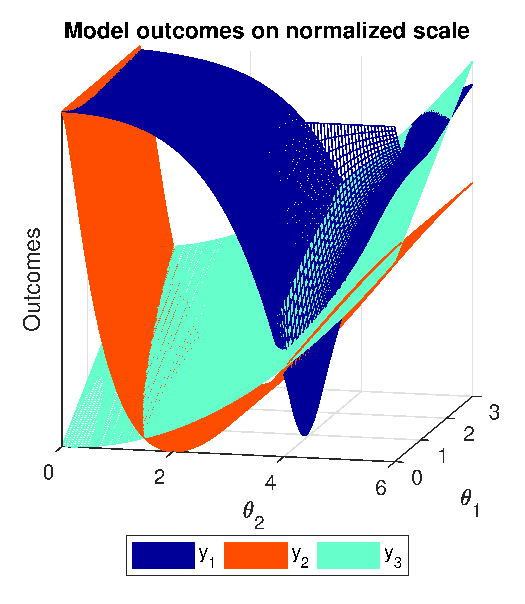
\includegraphics[width=.4\linewidth]{FIG_toy_sim_model_outputs}
\captionsetup{width=.4\linewidth}
\caption{Example model outputs shown on a common scale.}
\label{fig:toy_sim_outputs}
\end{figure}
%
%For CDO, the true function was used (rather than a GP emulator). 
%For CDO, a budget of 432 model observations was used. 
%%
%These were drawn as a full factorial design on a $3\times12\times12$ evenly-space grid over the supports of $x,\theta_1,\theta_2$. 
%%
%Using these model runs, the covariance function parameters $\lambda_\eta,\boldsymbol \beta^\eta$ in (\ref{eq:Hig_cov}) were set to their MLEs: $\lambda_\eta = 8.37\cdot10^{-4}$, $\boldsymbol\rho^\eta = [0.281, 0.999, 0.600, 0.720, 0.103]$ where $\rho^\eta_k = \exp(-\beta_k^\eta/4)$. 
%Thus we have 
Assuming an easily evaluated model, we have
%
\[
\mathbf y(\mathbf x, \boldsymbol\theta) = \mathbf f(\mathbf x,\boldsymbol \theta) + \delta(\mathbf x) + \epsilon
\]
%
for desired observation $\mathbf y$, where $\mathbf f$ is the model output, $\delta(\cdot)$ is the discrepancy function and $\epsilon$ is $N(0,0.05)$.

We initially set the desired observations to $[0,0,0]$, constant as a function of $x$. 
%
We then estimated the Pareto front via a preliminary round of CDO in order to estimate the standardized distance of the desired observation from the Pareto front.
%
The distance from the estimated Pareto front to the desired observation was found to be large -- at 16 units on the standardized scale, roughly four times the diameter of the entire model range.
%
As a result, the use of $[0,0,0]$ as a desired observation would lead to poor identifiability of the optimal region. 
%
This is because the desired observation is approximately the same distance from any point in the model range, relative to the distance from the desired observation to the optimal region.
%
%Therefore in order to improve identifiability of the optimal region, we updated the desired observation to lie closer to the estimated Pareto front (along the same line connecting to the orginal desired observation).
Therefore in order to improve identifiability of the optimal region, we updated the desired observation to lie along the same line connecting the original desired observation to the estimated Pareto front, but now closer to the latter.
%
We chose a distance of one unit away (roughly one fourth of the diameter of the model range), approaching the estimated Pareto front as closely as possible while remaining confident that the new desired observation of $[0.71, 0.71, 17.92]$ still outperforms the true Pareto front (i.e., lies outside the model range and is such that if it were added to the model range, it would be a Pareto optimal point).
%
We then set the discrepancy marginal precision $\lambda_\delta$ to 1 for subsequent CDO, corresponding to a degenerate prior informed by the estimated distance of the new desired observatino from the Pareto front.
%
Observation error $\epsilon(\cdot)$ from \eqref{eq:model_gen} was taken to be distributed as $N(0,0.05)$ for all $x$.
%
Figure \ref{fig:toy_sim_results} shows the results, including the marginal distributions of the calibration parameters. 
%
The sharply peaked marginals show substantial Bayesian learning compared to the uniform prior distributions on the calibration parameters. 
%
The calibration successfully maps the contours of the optimal region, and peaks near the true optimum. 
%
%Among the posterior predictive samples $\tilde {\mathbf y}$ associated with each draw of $\boldsymbol \theta$, $91.9\%$ lie within two standard deviations of the true optimum.

\begin{figure}
\centering
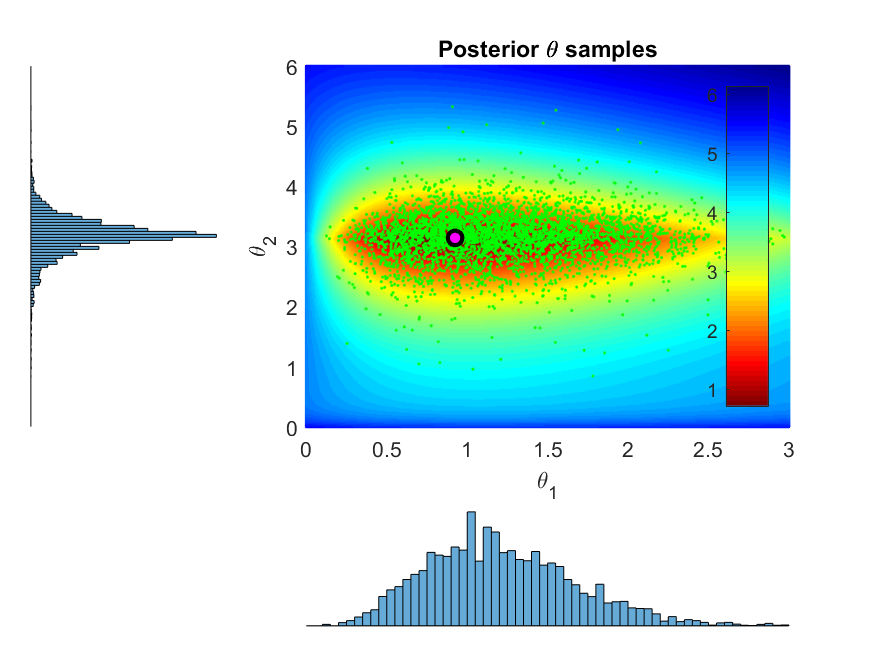
\includegraphics[width=.75\linewidth]{FIG_toy_sim_model_results}
\captionsetup{width=.75\linewidth}
\caption{Posterior draws from CDO in the simulated example. The heatmap shows, for each point in the parameter space, the Euclidean distance of the model output at that point from the desired observation (averaged across the control input range $[1.95,2.05]$). The purple dot shows the true optimum.}
\label{fig:toy_sim_results}
\end{figure}



\section{Application}\label{application}

In this section we describe the use of CDO for the problem of designing a material for constructing a wind turbine blade of fixed geometry. 
%
In traditional engineering design, material selection is a matter of choosing a material with appropriate properties for the project at hand from a database of known materials, often as a matter of ad-hoc satisficing. 
%
Material design usually occurs separately, and without an eye to specific end-uses. 
%
It is desirable to wed these design processes, selecting a material design by modeling its performance outcomes in a particular engineering application. 
%
Therefore, here we offer an example of calibrating material design parameters to desired performance targets for a wind turbine blade. 
%
This calibration is mediated by a model using \texttt{ANSYS} finite element analysis software. 
%
The finite element model is treated as an accurate representation of reality. %In this section I describe the emulator, and in Section \ref{MCMC} I describe its use for the calibration procedure.

\subsection{Project background}

Two primary performance targets for the design and construction of wind turbine blades are the distance (in meters) that the blade tip deflects under load from its starting position, and the angle of rotation the blade experiences under load.
%
Within the set of materials studied here, it is desirable that each of these measures be as close to zero as possible.
%
The blade is to be a composite of two given materials, one serving as the \textit{matrix} and the other the \textit{filler}. 
%
In a composite, the matrix holds the filler together; an example would be concrete, in which a filler of loose stones is combined with a matrix of cement.
%
For the wind turbine blade, given a fixed choice of matrix and filler, the properties of the composite depend on the volume fraction (i.e. the volume ratio of filler material to matrix material used in the composite) and the thickness of the material used to build the blade. 
%
The resulting material properties impact the performance of the blade, as well as its cost per square meter. 
%
We used CDO to find a distribution on optimal settings for volume fraction and filler.

The finite element model takes as inputs a triplet $(h,v,k)$, where $h$ is the operating temperature of the wind turbine (in kelvin), $v$ is the volume fraction of the material, and $k$ is the thickness of the material (in mm). 
%
The outputs of the model are a triplet $(d,r,c)$, where $d$ is tip deflection (in meters), $r$ is rotation (in radians), and $c$ is cost per square meter (USD). 
The wind turbine should be capable of operating over the range of temperatures 230K-330K. 
%
The goal of calibration is thus to find posterior distributions on $v$ and $k$ given outputs from the finite element simulator and desired observations.

\subsection{Emulation of finite element model}\label{emulator}
The finite element simulator is too computationally expensive to be suitable for direct use in (e.g.) an MCMC routine. 
%
Thus we employed a GP emulator in the manner of \cite{Williams2006}. 
%
For this purpose, we drew 504 (trivariate) observations from the finite element simulator. 
%
These inputs follow a Latin hypercube sampling design \citep{McKay1979} based on plausible ranges for the three inputs, as identified by expert opinion.
%
We consider the finite element observations to follow a GP with mean 0 and covariance function $C$ as described by (\ref{eq:Hig_cov}) above, with $\alpha_\eta=2$. 
%
This is equivalent to assuming smooth, infinitely differentiable sample paths. 
%
%I do not include a discrepancy function, per the considerations of Section \ref{obs_error}.

The hyperparameters $\lambda_\eta,\boldsymbol \beta^\eta$ must be estimated.
% 
For the reasons discussed in Section \ref{hyperparameter_estimation}, we estimated them prior to calibration to the desired observations, via maximum likelihood estimation.
% 
%Initially, a grid optimization method was used: a grid of $\boldsymbol \beta^\eta$ values was used, finding at each point of the grid the likelihood of the simulation observations integrated over the support of $\lambda_\eta$. 
%
%However, $\boldsymbol \beta^\eta$ is a five-dimensional vector, and a grid fine enough to be useful was too computationally burdensome to be feasible. Instead, a 
We used \texttt{fmincon()} in {\sc Matlab} %\citep{Cauchy1847} 
to maximize the log-likelihood of the simulation observations  (Equation \eqref{eq:full_dist} with $\mathcal D=\boldsymbol\eta$) over the joint (6-dimensional) support of $\boldsymbol \beta^\eta,\lambda_\eta$.  
%
The result is $\hat\lambda_\eta = 0.0152$, $\boldsymbol {\hat\rho}^\eta = (0.9358, 0.6509, 0.6736, 0.4797, 0.9673)$
%\begin{equation}\label{eq:MLEs}
%\boldsymbol {\hat\rho}^\eta = (0.9358, 0.6509, 0.6736, 0.4797, 0.9673),\quad
%\hat\lambda_\eta = 0.0152
%\end{equation}
where $\rho^\eta_k = \exp(-\beta_k^\eta/4)$. 
%A slice of the resulting emulator mean (for thickness = 20mm) for the tip deflection output is shown in Figure \ref{fig:emulator_surface}.

%\subsubsection{Wind turbine blade simulator}
%% Here the finite element model will be described
%Blah
%
%\subsubsection{Mathematical basis for the emulator}
%% Includes formulae for trained mean and covariance functions
%Blah
%
%\subsubsection{Experimental design}
%% How we selected the design points at which to observe the simulator
%Blah
%
%\subsubsection{Covariance parameters}
%% How they were selected
%Blah

%\paragraph{Finding covariance parameters via MCMC}
%% Why we didn't do it (computational difficulties
%Blah
%
%\paragraph{Grid optimization}
%% Advantages and disadvantages; full grid and integration of lambda
%Blah
%
%\paragraph{Gradient method}
%% Explanation and advantages
%Blah

%\begin{figure}
%\centering
%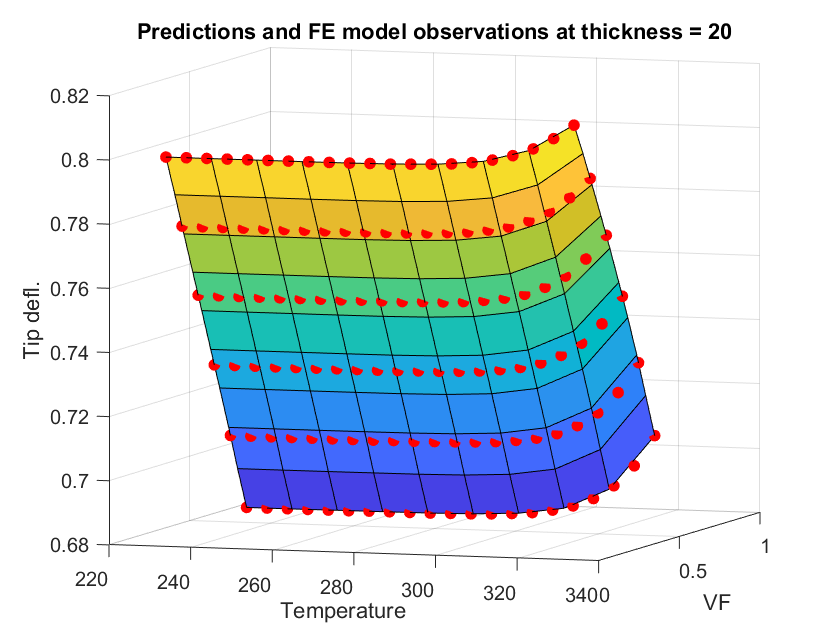
\includegraphics[width=.65\linewidth]{emulator_surface}
%\captionsetup{width=.65\linewidth}
%\caption{A slice of the GP emulator mean (restricted to the output for tip deflection) at thickness = 20mm. Red dots are observations from the simulator.}
%\label{fig:emulator_surface}
%\end{figure}

%\subsection{MCMC methods}
%% Background on MCMC
%Blah

\subsection{The model}\label{the_model}
% Choice of priors and resulting likelihood
Following the framework laid out in Section \ref{gaussian_processes} and the hyperparameters estimated in Section \ref{emulator}, the model takes the trained emulator to be distributed as
%
\begin{equation}\label{posterior_GP}
\mathcal {GP}\left(\mu^*(\mathbf b), C^*(\mathbf b,\mathbf b')\right)
\end{equation}
%
where $\mu^*(\mathbf b) = \mathbf C_{\mathbf b,\mathbf B} \cdot \mathbf C_{\mathbf B,\mathbf B}^{-1} \cdot \boldsymbol \eta$, $C^*(\mathbf b,\mathbf b') = \mathbf C_{(\mathbf b^T,\mathbf b'^T)^T,(\mathbf b^T,\mathbf b'^T)^T} - \mathbf C_{(\mathbf b^T,\mathbf b'^T)^T,\mathbf B}\cdot \mathbf C_{\mathbf B,\mathbf B}^{-1} \cdot \mathbf C_{\mathbf B,(\mathbf b^T,\mathbf b'^T)^T}$, $\mathbf C_{\Upsilon,\Gamma}$ is the matrix whose $i,j$ element is equal to the covariance between the observation at the $i^{\text{th}}$ row of $\Upsilon$ and at the $j^{\text{th}}$ row of $\Gamma$, $\mathbf b=(\mathbf x,\mathbf t)$ is a row vector of control and calibration inputs, $\mathbf B=(\mathbf b_1^T,\mathbf b_2^T,\cdots,\mathbf b_n^T)^T$ is the $1512\times5$ matrix of locations of the 1512 simulation observations, and $\boldsymbol\eta$ is a column vector of the 1512 simulation responses: $\eta_i=\eta(\mathbf b_i)$. 
%
All model inputs are normalized to [0,1] over their supports. All model outputs are standardized so that $\boldsymbol\eta$ has mean 0 and standard deviation 1.
%
$C(\cdot,\cdot)$ is given by (\ref{eq:Hig_cov}), where we plug in the MLEs given above. 
%
The full joint posterior density of the calibration parameters and discrepancy function hyperparameters, from \eqref{eq:full_dist}, is
\begin{equation} \label{eq:wt_full_dist}
\pi(\boldsymbol\theta,\lambda_\delta,\boldsymbol\rho^\delta|\mathcal D) 
\propto 
\pi(\mathcal D|\boldsymbol\theta,\lambda_\delta,\boldsymbol\rho^\delta)
\times
\pi(\lambda_\delta)
\times
\pi(\boldsymbol\rho^\delta).
\end{equation}
%

The initial desired observations were set to $[0,0,0]$, constant as a function of temperature, on a grid of temperature values.
%
We carried out an initial round of CDO in order to update the desired observations to ones that lie an estimated distance of 1 (on a standardized scale) from the Pareto front.
%
A total of 20,000 samples were drawn via Metropolis-Hastings-within-Gibbs MCMC, of which 4,000 samples were discarded as burn-in. 
%
During the burn-in period, the covariance of the proposal distributions for $\boldsymbol \theta$, $\lambda_\delta$, and $\boldsymbol\rho^\delta$ were all periodically adjusted for optimal acceptance rates using the sample covariance of the preceding draws.
%
%The adjustment took place every 100 iterations of the MCMC, at which point the relevant covariance matrix was set to be equal to the sample covariance of the previous draws, times a scalar multiplier. 
%
%The level of the scalar multiplier was adaptively adjusted to promote optimal acceptance rates of $\approx 30\%$ for $\boldsymbol\theta$ and $\boldsymbol\rho$, and $\approx 44\%$ for $\lambda_\delta$.
%
As expected for the preliminary round of CDO, the posterior distribution of $\boldsymbol\theta$ was quite diffuse.
%
We used the GP emulator to estimate the model output for each sample of $\boldsymbol \theta$ drawn.
%
We filtered the resulting posterior predictions to retain only the estimated Pareto front.
%
Examining the estimated Pareto front, one finds a distinct ``elbow''; see figure \ref{fig:elbow}.
%
\begin{figure}
\centering
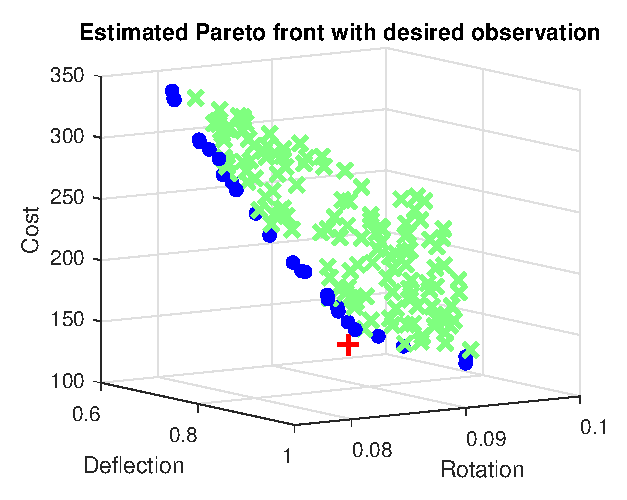
\includegraphics[width=.7\linewidth]{FIG_est_PF_with_des_obs}
\captionsetup{width=.7\linewidth}
\caption{The green points show the estimated range of the model. The blue points show the estimated Pareto front. The red dot is the desired observation selected to calibrate to the ``elbow'' in the Pareto front.}
\label{fig:elbow}
\end{figure}
%
We selected this elbow as the target for calibration.
%
To do so, we set the point $[\mathrm{deflection}=0.75\mathrm m,\ 
\mathrm{rotation}=0.09\ \mathrm{rad},\ 
\mathrm{cost}=\$130.34]$
 as the desired observation (constant as a function of temperature).
%
The elbow is the closest region of the Pareto front to this point.
%
Based on the estimated Pareto front, the desired observation is approximately 0.2 units away on the standardized scale.
%
Therefore, we set $\lambda_\delta=1/0.2^2=25.$
%

In the resulting CDO, we employed the same MCMC approach as in the preliminary round, except that $\lambda_\delta$ was now treated as known.
%
The marginal posterior distributions are shown in Figure \ref{fig:wt_marg_post}, along with the (uniform) prior distributions. 
%
\begin{figure}
\centering
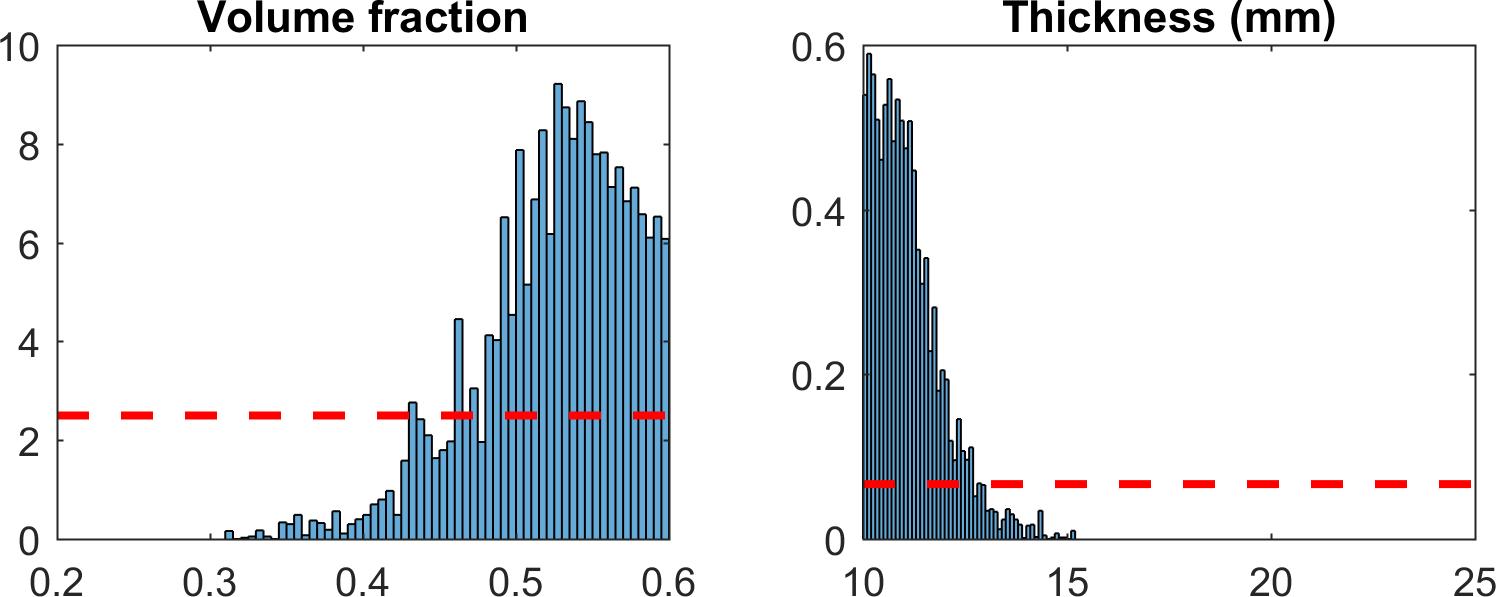
\includegraphics[width=.7\linewidth]{FIG_posterior_marginals_with_priors}
\captionsetup{width=.7\linewidth}
\caption{The histograms show the marginal posterior of each calibration parameter. The dotted lines show the priors.}
\label{fig:wt_marg_post}
\end{figure}
%
The mean model output under the prior is $[\text{deflection}=0.76\mathrm m,\ \text{rotation}=0.09\text{ rads},\ \text{cost}=\$207.90/\mathrm m^2]$, whereas under the posterior it is $[0.76\mathrm m,0.09\ \mathrm{rad},\$148.68]$.
%
Though the performance outcomes are approximately the same under the posterior distribution as under the prior, the cost per square meter has dropped dramatically.
%
If one desires to prioritize gains in performance over cost, this can be accomplished by selecting desired observations that reflect those priorities. 

\subsection{Pareto front estimation}\label{removing_cal_pars}

%\subsubsection{Motivation}

Often in the case of a system with multivariate output, one might not antecedently have a clear target outcome.
%
When \textit{ceteris paribus} all outputs are to be minimized, any point in the Pareto front is optimal relative to some set of priorities.
%
If those priorities have not been explicitly determined prior to calibration, then no particular outcome can be targeted.
%
In determining one's priorities, it is helpful to know the Pareto front of the relevant system.
%
For example, in a system where quality is monotonically increasing in cost, depending on one's tolerance for high cost any point in the model range might be optimal.
%
In determining one's priorities and selecting a target outcome, it is valuable to have a clear and accurate understanding of the Pareto front of the system.
%
In low-dimensional cases, CDO may be used to achieve such a holistic picture of the Pareto front by optimizing to each of a grid of performance targets.
%
%Where a model contains several outputs that one wishes to optimize, it can become complicated to juggle one's priorities in selecting targets for each of these outputs.
%
%Again to speak from the wind turbine application: we know we want to keep cost, deflection, and rotation low, but we might not have a clear prior conception of exactly what sorts of trade-offs amongst those outcomes we would consider optimal, much less how to implement our priorities in the calibration procedure. 
%
%Rather than wishing to optimize relative to some particular set of desired observations, one may prefer simply to learn as much as possible about the Pareto front as a whole.
%
%In low-dimensional cases this may be achieved using CDO as follows.
%
To do this, where the model output is $d-$dimensional, one may draw a grid over the range of $d-1$ of the model outputs and perform CDO to minimize the remaining output at each point of the grid.
%
The $d-1$ outputs, at each grid point, are treated as known up to observation error (meaning that the discrepancy function $\delta(\cdot)$ is set to 0 in the dimension of these outputs).
%
The resulting estimate is distinguished from other methods of estimating the Pareto front (including from the filtering method employed in preliminary CDO) by including uncertainty quantification.
%

This procedure is illustrated here using the wind turbine blade application.
%
For simplicity, rotation has been removed as a model output, leaving a system with 2-dimensional output of deflection and cost. 
%
The range of cost is known (via preliminary CDO) to be $[\$96,\$352]$.
%
A 20-point grid was drawn over this range of costs. 
%
%Using the rough estimate of the Pareto front from preliminary CDO, we found that to cover the Pareto front, the cost grid should cover the range $[\$96,\$352]$.
%
For each point $c$ in the cost grid, we used the point $(0\mathrm m,\$c)$ as the performance target for calibration (constant with respect to temperature).
%
For each such point, then updated this initial desired observation to improve identifiability using the rough estimate of the Pareto front from preliminary CDO using desired observation $(0\mathrm m,\$0)$.
%
Note that only one round of preliminary CDO was needed for this purpose, rather than a separate instance at each grid point.
%
%, to be a point which lies near the Pareto front, to improve identifiability.
%
%Here as in Section \ref{the_model}, ``near'' was taken to be 0.2 units on the standardized scale of model outputs.
%

%\paragraph{Specifying known cost}\label{known_cost}
%
%The above strategy of performing the calibration across a grid and forming a response surface over that grid may be applied even more directly, to largely the same end as in the previous section. Namely: rather than replace one or more desired outputs with a prior on the calibration inputs and drawing a grid over the hyperparameter(s) of that prior, one can instead simply draw a grid over one or more of the desired outputs, treating those outputs as known up to slight deviations at each point of the grid. This strategy has the advantage that, unlike the above strategy, it does not require that we have prior knowledge of any relationship between the calibration parameters and the outputs. Furthermore, whereas the previous strategy requires removing a model output, the current strategy uses the same version of the model, relying solely on changes to the desired observations and observation variance to effect the strategy. In comparison with the previous section's strategy, the approach in the current section also enjoys better interpretability.
%
%For convenience, call an output that is specified as known up to slight deviations in the way suggested here ``d-known''. To specify an output as d-known, it suffices to (1) choose a desired observation of that output which is realistically achievable, and (2) set a constant, low observation variance for that output. The precise value of the observation variance for a d-known output can be tuned during the burn-in period of the MCMC routine. It ought to be as low as possible while still allowing for healthy mixing in the MCMC. If the variance is too small, then proposed draws of the calibration parameters will be likely to take the model output too far away from the d-known output, resulting in the draw being rejected, and hence low acceptance rates and poor mixing.
%
%The other desired observations -- those that are not d-known -- can be treated as usual, with their observation variances each drawn from a $1/\sigma^2_i$ prior, or whichever other treatment of observation variance from Section \ref{des_obs_var} one wishes to use. Thus at the calibration procedure which takes place at each point in the grid of d-known outputs, the d-known outputs have in essence been removed from the CDO, and are treated as known up to a slight variance for facilitating healthy MCMC. This ``removal'' requires little modification to the model, but still serves to simplify the choice of desired observations and observation variance. 
%
%The full model is given by
%\begin{equation}\label{full_model_3}
%\begin{aligned}
%\pi(\boldsymbol\theta,\mathbf C_{\mathbf y}|\mathcal D ) &\propto
%\pi(\mathcal D|\boldsymbol\theta,\mathbf C_{\mathbf y}) \times \pi(\boldsymbol\theta) \times \pi(\mathbf C_{\mathbf y})\\
%&\propto  \pi(\mathcal D|\boldsymbol\theta,\mathbf C_{\mathbf y}) \times \pi(\mathbf C_{\mathbf y})\\
%&\propto \lvert \mathbf C_{\mathcal D} \rvert ^{-1/2} \mathrm{exp}(\mathcal D^T \mathbf C_{\mathcal D}^{-1} \mathcal D) \times \prod_{i=1}^2 \frac1{\sigma^2_i}
%\end{aligned}
%\end{equation}
%where $\mathbf C_{\mathbf y}$ is the diagonal matrix where the $j,j$ entry $c_j$ is equal to $\sigma^2_1$ if $y_j$ is an observation of deflection, $c_j=\sigma^2_2$ if $y_j$ is an observation of rotation, and $c_j = s$ if $y_j$ is an observation of cost, for some small pre-selected value of $s$. In this application, I set $s=0.05$, so that the observation variance on standardized cost values at each point of the grid was 0.05. 

%The result of this strategy is similar to that one can derive a response surface over the $d-1$-dimensional grid of outputs, where that response describes the optimal results across the grid. 
%
%If the grid covers the Pareto front in $d-1$ dimensions, then t
The result of the strategy is to provide an estimate of the response surface with included uncertainty quantification describing, for each point in the grid, the optimal achievable outcome for the output not included in the grid.
%
Thus a decisionmaker can visualize the space of desirable possibilities with associated uncertainty metrics. 
%
They can do so without the need for antecedently rigorously determining their exact priorities for weighing gains in each of the outputs against one another.
%, nor (much worse) working out how to translate those priorities into specific choices of desired observations and observation variance schemes. 
%This is similar to the strategy of the previous section, but in addition to other benefits, this result has better interpretability in that the grid is over one of the model outputs, rather than over a hyperparameter whose interpretation is somewhat dubious. For example, a decision-maker is likely to feel quite comfortable choosing a budget based on expected outcomes at each cost; they may be less comfortable selecting a value of $\lambda_{cost}$.

%The same sort of uncertainty analysis described in Section \ref{non-uniform_prior} is available here, since posterior parameter uncertainty and code uncertainty are easily recovered from the results of the MCMC routine. 
%
The result of applying this strategy to the wind turbine blade application is shown in Figure \ref{fig:known_cost}. 
%
The rightmost plot is included to verify that the posterior model output respected the d-known cost values used in the calibrations.
%
The Pareto front for the system appears with uncertainty bands in the righthand plot.
%
This plot visualizes a distribution on the optimal performance outcome for any cost that a decisionmaker might select as a budget for production, which would be helpful when selecting a budget.
%
For example, the elbow around \$140 manifests itself as a potentially attractive choice, since it can be seen in the plot that prior to that point each dollar spent brings significant gains in reducing deflection.
%
Spending above that level continues to reduce deflection, but less sharply.


\begin{figure}
\centering
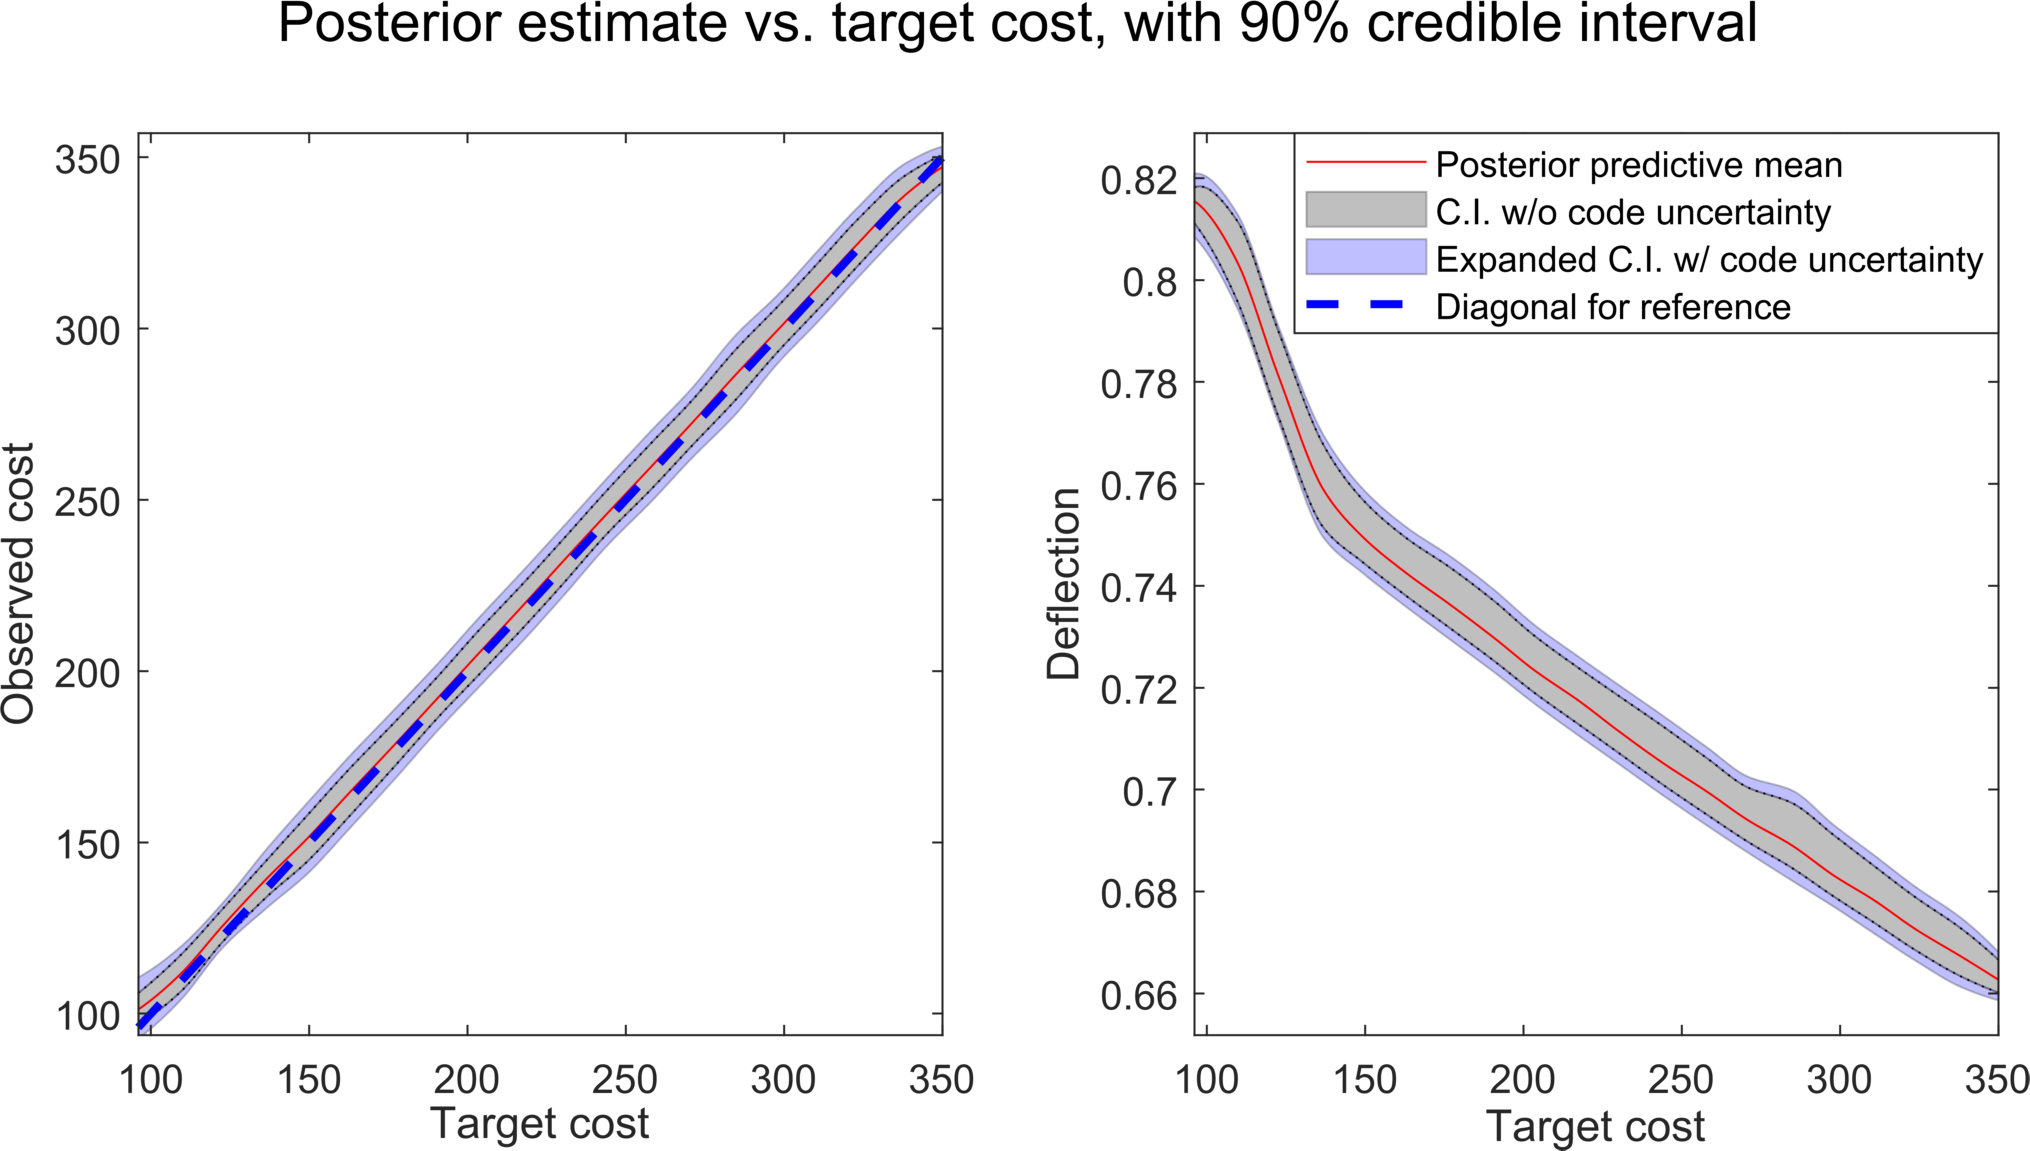
\includegraphics[width=.8\linewidth]{FIG_cost_grid_pareto_bands}
\captionsetup{width=.8\linewidth}
\caption{``Pareto bands'' of wind turbine blade posterior cost and tip deflection across a range of target costs. The gray region gives a 90\% credible interval only considering parameter uncertainty; the blue region extends this to include code uncertainty.}
\label{fig:known_cost}
\end{figure}




\section{Conclusion} \label{conclusion}
% Discussion of the role of computer model validation as a potential methodology for design

In this work we have described the 
%theoretical background for the use of Gaussian processes to emulate computationally expensive computer model code, and the 
use of computer model calibration under the framework established by \cite{Kennedy2001}, \cite{Williams2006} and \cite{Bayarri2007} and how it can be used to address questions of engineering design. 
%
CDO is a modification of that framework which calibrates a computer model, not to field observations, but rather to desired observations; i.e., performance targets for the system. 
%
Unlike other methods of Bayesian optimization (e.g., \citealt{Shahriari2016}), CDO does not require the ability to carry out computer model observations adaptively.
%
Instead, it can operate using a batch of observations gathered prior to (and independently of) the calibration procedure.
%
We described the implementation of this approach in an MCMC routine along with considerations to accommodate computational instability.
%
The use of this methodology is illustrated in the case of material design for a wind turbine blade. 

We have shown thereby a variety of ways in which CDO can be used to guide decision-makers in the design process. 
%
By expropriating established tools of model calibration, CDO offers a method of optimization which is sensitive to all sources of uncertainty, and which results in an estimate that includes uncertainty quantification.

As discussed earlier, the methodology as described here treats the computer model as universally valid over the domain of the calibration inputs. 
%
Future work in this area will include the use of a discrepancy term capturing model bias.
%
This would allow for simultaneous calibrations: both traditional and CDO.
%
That is, a computer model could be calibrated to real observations while also being calibrated to performance targets treated as desired observations.
%
These two goals would not necessarily conflict, since the two calibrations take different inputs as the calibration parameters.
% 
CDO calibrates inputs that are under operator control, and thereby would be treated as control inputs in traditional calibration.
%
Other extensions of the proposed methodology could include its application to state-aware calibration \citep{Atamturktur2015,Stevens2018,Brown2016}, which would allow the optimal region of the calibration parameters to vary as a function of the control inputs.



\bibliographystyle{apalike}

\pagebreak

\bibliography{lit_review}


\end{document}


%Generalizing from \cite{Kennedy2006}, I expand the Bayesian analysis to include the diagonal observation variance matrix $\mathbf C_{\mathbf y}$, rather than requiring this value to be specified as known, and I allow for a non-uniform prior $\pi(\boldsymbol \theta)$ on the calibration parameters. By (\ref{eq:full_dist}) on page \pageref{eq:full_dist}, 
%since I estimate $\boldsymbol \rho^\eta,\lambda_\eta$ by maximum likelihood, set $c=0$, and do not include a discrepancy function, we have for desired observations $\mathbf y=(y (b_{n+1}),\cdots,y(b_{n+m}))^T$ and $\mathcal D=(\mathbf y^T, \boldsymbol\eta^T)^T$:
%\begin{equation}\label{eq:the_model}
%\pi(\boldsymbol \theta,\mathbf C_{\mathbf y}|\mathcal D) \propto \pi (\mathcal D|\boldsymbol \theta,\mathbf C_{\mathbf y})\times \pi(\boldsymbol \theta)\times \pi(\mathbf C_{\mathbf y})
%\end{equation}
%and $\mathcal D|\boldsymbol \theta,\mathbf C_{\mathbf y} \sim N(\boldsymbol 0_{m+n}, \mathbf C_{\mathcal D})$, 
%\begin{equation}\label{eq:the_covariance}
%\mathbf C_{\mathcal D} = \mathbf C_{\boldsymbol\eta} + 
%\begin{bmatrix}
%\mathbf C_{\mathbf y} & \boldsymbol 0\\ 
%\boldsymbol 0 & \boldsymbol 0
%\end{bmatrix}
%\end{equation}
%where $\mathbf C_{\boldsymbol\eta}$ is a $(m+n)\times(m+n)$ matrix with $i,j$ entry $C(b_i,b_j)$.
%
%The model as described above leaves open several details of the model, options for which are explored in the remainder of Section \ref{MCMC}. In \ref{des_obs_var} I consider options for $\pi(\mathbf C_{\mathbf y})$, the prior on observation variance, including setting a degenerate prior corresponding to specifying a known observation variance. In \ref{which_data} I take up the question of which data one ought to desire, showing how the goals of one's analysis can support vastly different choices for desired data. In \ref{removing_cal_pars} I explore options for $\pi(\boldsymbol \theta)$, the prior on the calibration parameters. I depart thereby from the framework of \cite{Kennedy2006}, who (implicitly) restrict the calibration model to the case of using a uniform prior. An example is used to show how setting a non-uniform prior here can allow one to reduce the number of parameters that are subjected to calibration in the model. Before taking up these matters, in \ref{convergence_difficulties} I take up convergence difficulties that arise due to boundary constraints on the calibration parameters.
%\subsubsection{Full model and likelihood}
%Blah
%
%\subsection{Convergence difficulties}\label{convergence_difficulties}
%% And the idea to eliminate boundary constraints
%As will often be the case in calibration problems, in the application considered here the calibration parameters $(v,k)$ have compact support: $v\in [.1,.6],$ $k\in [10\mathrm{mm},25\mathrm{mm}]$.
%%DISCUSS Andrew asks "Is compact support necessary? For the sake of posterior inference, it seems to me that one could do just as well with open parameter sets." I'm not sure what he means: is he suggesting that reparameterization to open sets is possible? Or that ignoring the boundaries is? Or something else? And either way, how does it affect the point made here?
%When the calibration procedure leads to draws near these boundaries, the MCMC routine may suffer poor mixing. For example, consider using proposal density $q$ such that $(v^*,k^*)\sim N((v^{(i)},k^{(i)}),\Sigma)$ for some proposal covariance $\Sigma$. 
%The symmetry of a normal proposal density makes it convenient for MCMC, but also exacerbates the difficulties that come from boundary conditions. 
%Using such a proposal density with $\pi(\boldsymbol \theta)$ a uniform density on the support of $\boldsymbol \theta$ amounts to simply discarding any proposed draw of $(v,k)$ that falls outside of the boundaries for those variables. 
%This is inefficient, as it leads to low acceptance rates during MCMC for new draws of $\boldsymbol \theta$. 
%When a new proposed draw is rejected, the previous draw is repeated, leading to extremely high levels of autocorrelation in the MCMC draws.
%
%%DISCUSS What are some sources for reflecting boundary proposals?
%
%There are several ways to tackle this problem. 
%One approach seeks to improve acceptance rates through utilizing an adaptive proposal covariance magnitude, so that $\Sigma$ is periodically updated during the burn-in period in order to achieve an optimal acceptance ratio of around 23\%; see \cite{Roberts1997}. 
%If $\Sigma$ is diagonal, then this is especially simple to implement. 
%One simply keeps track of the number of times that a proposed draw of $\theta_i$ is outside of its boundaries, and then every 100 MCMC steps or so, if the number of out-of-boundary proposals exceeds a specified threshold, then one reduces $\Sigma_i$, the proposal variance of $\theta_i$. 
%This strategy can easily be paired with a more comprehensive adapative proposal covariance -- e.g., one that is set to increase in magnitude whenever more than 30 of the most recent 100 draws have been accepted, and decrease in magnitude whenever fewer than 20 of the most recent draws have been accepted. 
%If the posterior distribution is merely near the boundary, such measures may suffice; however, in calibration to desired observations (which tend to be extreme outliers \textit{qua} observations), often the calibration parameters will be drawn strongly to the boundaries, and in such a situation the sort of adaptive proposal distribution described above may be insufficient to secure good acceptance ratios. 
%
%A second strategy is to use an independence chain approach \citep{Tierney1994}, in which the proposal density is independent of all previous draws. E.g., for compact support $\mathcal S$, one could simply draw new proposals as uniform over $\mathcal S$. When the posterior distribution is diffuse over its support, this can be effective. Otherwise, it can lead to low acceptance rates, as too many proposals are generated in low-density areas of the posterior distribution. 
%
%A third strategy would be to transform the variables to be unbounded. This requires describing the model in terms of these transformed variables. An adaptive covariance can be used here as well, further improving acceptance rates. A fourth, closely related strategy would be to employ some variety of proposal with the same support as the variables. Indeed, the difference between the third and fourth strategies is largely conceptual. Consider, for example, using the logit transform to remove boundary constraints from variables with compact support. Without boundary constraints, one can recover the convenience of a symmetric, Gaussian proposal distribution, without risk of proposing outside of the variables' support. But in addition to being viewed as a symmetric distribution on the transformed variables, this can equally be viewed as a non-symmetric distribution on the untransformed variables. I apply this logit transform to $(v,k)$ in the wind turbine application, where for convenience I adopt the latter conceptual perspective. 
%
%The adaptive proposal strategy sketched above changes only the magnitude of the proposal covariance, and depends upon having a diagonal covariance matrix. This diagonality is what allows the easy modification of the magnitude of the variance of all and only those parameters which are being drawn outside of their boundary constraints. But where boundary constraints are no longer a problem, it is just as convenient to establish a non-diagonal proposal covariance. This will, of course, be of especially high value when the calibration parameters are correlated in the posterior distribution, which is frequently the case. Thus, when updating the proposal covariance, one can set it to be equal to the sample covariance of the unique samples accepted thus far in the MCMC routine.
%
%%In the case of compact support, using the logit transform on the normalized variable removes the boundary constraints. Without boundary constraints, one can recover the convenience of a symmetric proposal, such as a normal distribution. An adaptive proposal covariance further aids strong mixing here. The adaptive proposal strategy sketched above depends upon having a diagonal proposal covariance matrix for the calibration parameters; this is what allows the easy modification of the magnitude of the variance of all and only those parameters which are being drawn outside of their boundary constraints. But where boundary constraints are no longer a problem, it is just as convenient to establish a non-diagonal proposal covariance. This will, of course, be of especially high value when the calibration parameters are correlated in the posterior distribution, which is frequently the case in our application. Thus, when updating the proposal covariance, one can set it to be equal to the sample covariance of the unique samples accepted thus far in the MCMC routine. 
%
%
%If the acceptance ratio is low early in the MCMC when using this adaptive technique, the resulting proposal covariance may be too small. To promote more efficient exploration of the parameter space, the covariance can be multiplied by a constant $\tau$ which is also updated whenever the proposal covariance is updated. One may adjust $\tau$ so as to induce acceptance rates close to 23\%. Thus, during the burn-in period, every $n_0$ draws (with $n_0$ set to, e.g., 100), the proposal covariance $\Sigma$ and multiplier $\tau$ are updated to $\Sigma^*$ and $\tau^*$ as follows, where $a$ is the proportion of the past $n_0$ draws that were accepted, $I$ is the indicator function, and $\mathbf S$ is the set of all samples drawn so far:
%\begin{equation}
%\begin{aligned}
%\tau^* &= \tau \cdot (1.25  I(a>25) + 0.75 I(a<20))\\
%\Sigma^* &= \tau^* \cdot \mathrm{Cov}(\mathbf S)
%\end{aligned}
%\end{equation}
%
%%More cautiously (lest the proposal covariance become unduly influenced by early, nonrepresentative draws) but in the same spirit, one can proceed as follows. Set the proposal covariance to begin as some pre-specified, diffuse covariance (such as the identity $I$). Periodically update to a weighted mixture of the previous covariance matrix with the sample covariance of the most recent 50\% of the unique samples drawn in the MCMC routine, where the weight increases to favor the sample covariance over the course of the burn-in period. Furthermore, a scalar multiplier $\tau$ of the proposal covariance can be adjusted so as to induce acceptance rates close to 23\%. This strategy was found to be most successful in our application. Thus where the first $g$ samples are treated as burn-in, each time the proposal covariance $\Sigma$ and multiplier $\tau$ are updated to $\Sigma^*$ and $\tau^*$ at the $r^{\text{th} }$ iteration:
%%\begin{equation}
%%\tau^* =  \tau \left ( 0.9 \cdot I(a<0.2) + 1.1 \cdot I(a>0.3)\right),\quad
%%\Sigma^* = \tau^* \left (  
%%\frac{g-r}\rho \Sigma + \frac r g C_U \right)
%%\end{equation}
%%where $I(\cdot)$ is the indicator function, $a$ is the acceptance rate from recent (e.g. previous 100) draws, and $C_U$ is the sample covariance of the most recent half of all unique samples drawn in the MCMC routine.
%
%The adaptation takes place only during the burn-in period. 
%As a result, the adaptive nature of the algorithm does not change the fact that it is an implementation of the Metropolis-Hastings algorithm given in \cite{Hastings1970}. Hence it is guaranteed to converge to the target distribution. 
%However, another option would be to employ the adaptive Metropolis schema of \cite{Haario2001,Haario2005,Haario2006}, who continue to update the proposal covariance to be the sample covariance of all previous draws throughout the sampling procedure (up to a scaling constant which, unlike $\tau$ above, is not itself adaptive). This sampling method loses the Markov property and hence is not an MCMC method. 
%Nonetheless the authors show it is ergodic under the conditions that the target distribution is bounded with bounded support. 
%
%Recall (from Section \ref{MCMC_methods}) that abandoning symmetry in one's proposal distribution requires that one employ the more general Metropolis-Hastings algorithm, rather than the Metropolis algorithm of \cite{Metropolis1953}. Interpreting a normal distribution on the logit-transformed variables as a distribution on the original variables, it is not symmetric. Therefore, calculate the log acceptance probability a proposal for the $i^{\text{th}}$ draw of $\boldsymbol \theta$ as 
%\begin{equation}
%\log \alpha = \log(\boldsymbol \theta^*|\mathcal D, \mathbf C_{\mathbf y}) - \log(\boldsymbol \theta^{(i-1)}|\mathcal D,\mathbf C_{\mathbf y}) + \log q(\boldsymbol \theta^{(i-1)}|\boldsymbol \theta^*)
%- \log q(\theta^* |\boldsymbol \theta^{(i-1)})
%\end{equation}
%where the use of the log scale is required in order to avoid significant round-off and underflow errors due to the dimensionality of $\mathcal D$.
%
%The benefits of the logit-transformed, unbounded proposal over a version of the MCMC using a normal proposal (with adaptive covariance) over the untransformed calibration parameters are displayed in Figure \ref{ACFs}. Sizeable autocorrelation appears in the untransformed version, whereas in the logit-transformed version the autocorrelation drops off to insignificance within about 30 steps.
%
%\begin{figure}
%\centering
%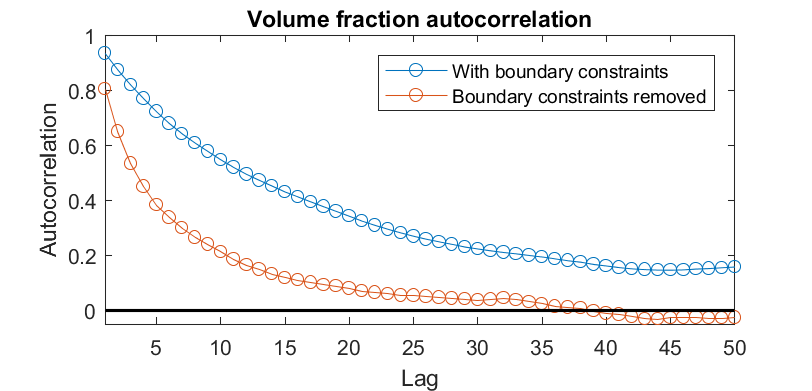
\includegraphics[width=.65\linewidth]{ACF_bnd_cnds_fig}
%\captionsetup{width=.65\linewidth}
%\caption{Auto-correlation for draws both with and without the elimination of boundary conditions.}
%\label{ACFs}
%\end{figure}

%\subsection{Desired observation variance}\label{des_obs_var}
%% 4 versions: heterosked constant, homosked constant, heterosked prior, homosked prior
%In the framework of \cite{Kennedy2006} on which much of the current approach is based, observation variance is assumed to be known. 
%That assumption is less straightforward in the case of CDO. 
%However, as explained below, there are applications in which setting a ``known'' observation variance is appropriate. 
%In this section, I consider the option of specifying observation variance versus setting a (non-degenerate) prior on observation variance. 
%I also consider the option of whether to set different observation variances for different outputs, or a single observation variance on all (standardized) outputs. 
%Table \ref{table:obs_vvar_comp} and the corresponding Figure \ref{fig:comp_obs_var} of MCMC results show how impactful are the choices amongst these options in the wind turbine blade design application. 
%The posterior mean model output varies significantly across the four available strategies, which correspond to different specifications of observation variance settings. 
%The table reflects the choices of (1) whether to specify that the observations are homoskedastic with respect to output type (e.g., whether standardized cost output has the same observation variance as standardized deflection output), and (2) whether the observation variance is set to a constant level or given a (nondegenerate) prior.
%From \eqref{eq:the_model} above, the full models corresponding to these choices, assuming a uniform prior on the calibration parameters, are as follows. 
%Columns one and two of the table both correspond to specifying $\boldsymbol \sigma = (\sigma^2_1,\sigma^2_2,\sigma^2_3)^T$ as the observation variance for each of the three outputs. 
%The two columns differ only in the value of $\boldsymbol \sigma$. 
%The prior $\pi(\mathbf C_{\mathbf y})$ in \eqref{eq:the_model} is thus the degenerate prior $\delta_{\boldsymbol\sigma}(\cdot)$, the Dirac delta function centered at $\boldsymbol \sigma$. 
%Here, $\mathbf C_{\mathbf y}$ is a diagonal matrix where the $i,i$ entry is equal to $\sigma^2_j$ iff desired observation $y_i$ is an observation of output $j$. 
%E.g., if $y_4$ is an observation of rotation, then the fourth diagonal element of $\mathbf C_{\mathbf y}$ is $\sigma^2_2$, the observation variance for rotation. 
%So for these two columns the full model is given by:
%\begin{equation}\label{eq:full_model_1}
%\begin{aligned}
%\pi(\boldsymbol\theta,\mathbf C_{\mathbf y}|\mathcal D) &\propto \pi(\mathcal D|\boldsymbol\theta,\mathbf C_{\mathbf y}) \times \pi(\boldsymbol\theta) \times \pi(\mathbf C_{\mathbf y})\\
%&\propto \pi(\mathcal D|\boldsymbol\theta,\mathbf C_{\mathbf y}) \\
%&\propto \lvert \mathbf C_{\mathcal D} \rvert ^{-1/2} \mathrm{exp}(\mathcal D^T \mathbf C_{\mathcal D}^{-1} \mathcal D)
%\end{aligned}
%\end{equation}
%where $\mathbf C_{\mathcal D}$ is given in \eqref{eq:the_covariance}, and where in the final expression I do not explicitly include the uniform $\pi(\boldsymbol\theta)$ or the degenerate $\pi(\mathbf C_{\mathbf y})$.
%Columns three and four each place a prior distribution on the observation variances. Column three places independent priors $1/\sigma^2_i$ on each of the $\sigma^2_i$, $i=1,2,3$, which serve as the observation variances of the three outputs. Column four places a single prior $1/\sigma^2_1$ on a scalar value $\sigma^2_1$ which serves as the observation variance for each of the three outputs. Thus the full models for these columns are:
%\begin{equation}\label{eq:full_model_2}
%\begin{aligned}
%\pi(\boldsymbol\theta,\mathbf C_{\mathbf y}|\mathcal D ) &\propto
%\pi(\mathcal D|\boldsymbol\theta,\mathbf C_{\mathbf y}) \times \pi(\boldsymbol\theta) \times \pi(\mathbf C_{\mathbf y})\\
%&\propto  \pi(\mathcal D|\boldsymbol\theta,\mathbf C_{\mathbf y}) \times \pi(\mathbf C_{\mathbf y})\\
%&\propto \lvert \mathbf C_{\mathcal D} \rvert ^{-1/2} \mathrm{exp}(\mathcal D^T \mathbf C_{\mathcal D}^{-1} \mathcal D) \times \prod_{i=1}^k \frac1{\sigma^2_i}
%\end{aligned}
%\end{equation}
%where for column three $k=3$ and $\mathbf C_{\mathbf y}$ is defined as in columns one and two, and for column four $k=1$ and $\mathbf C_{\mathbf y}=\sigma^2_1 \mathbf I_{m\times m}$. In both cases, the final expression does not explicitly include the uniform $\pi(\boldsymbol\theta)$.
%
%Notice in Table \ref{table:obs_vvar_comp} that column three is noticeably distinct from the others. Here is the only case in which the MCMC is free to alter the \emph{proportions} of observation variance allotted to the various outputs. In this case, the desired observation was essentially achieved for deflection and rotation, whereas the posterior cost was far from the desired cost. Thus, using the settings reflected in column three, we are able to learn that it is ``easier'' to achieve these two performance metrics than to achieve the cost target.
%
%When CDO is used without a discrepancy function and with observation variance sampled under a prior, the posterior distribution on observation variance amounts to an indirect measure of how closely reality can approximate our desired observations. E.g., from the fact that posterior observation variance from the routine represented in column three of Table \ref{table:obs_vvar_comp} was near zero, we see immediately that the cost target was achieved. Likewise, extremely high posterior observation variance indicates that the target could not be achieved. The posterior distribution reflects the (false) assumption that the difference between the desired observations and the true system mean is accounted for by random, mean-zero noise. 
%
%Matters are different when a set observation variance is specified for each output. Clearly, since the observation variance isn't sampled in the MCMC, there is no Bayesian learning to be had here. However, there is an opportunity to specify priorities through the specification of the variance. When the desired observations are outside the range of what is realistically achievable, the specific level of the observation variance is unlikely to matter much (unless it is so low as to engender computational difficulties). More important (in the case of multivariate output) is the fact that in specifying the observation variance, one is implicitly specifying the relative importance of each output. E.g., if I set a very diffuse observation variance on cost, and a very small one on deflection, then I have told the model that reduction in deflection is to be prioritized over reduction in cost. Whether one chooses to do so will depend on one's goals in calibration, as well as one's level of prior knowledge as to how close to reality one's desired observations are.
%
%Such prioritization can be harnessed to achieve calibration goals in ways that will be explored in Section \ref{removing_cal_pars}. There, one essentially sets the observation variance for all and only those parameters that one \emph{ceases} to treat as calibration parameters. In general, since there is no true value of the observation variance, it is better to let the data inform us about $\mathbf C_{\mathbf y}$: setting a scale-invariant $1/\sigma_i^2$ prior on each diagonal element $\sigma_i^2$ of $\mathbf C_{\mathbf y}$ yields posterior values of $\mathbf C_{\mathbf y}$ that inform us as to how achievable our desired observations are.
%
%There is another lesson to be derived from Table \ref{table:obs_vvar_comp}; namely, a warning that it is important to be aware of the impact of correlated outputs on the calibration procedure. Notice from the third column of the table that the posterior mean output almost achieves the desired observation for deflection and rotation, at the expense of falling wildly short on cost. However, it is known that the true model can achieve the desired cost of \$96/m$^2$ (for high levels of deflection and rotation). Part of what makes this outcome possible is that deflection and rotation are strongly positively correlated with each other, and negatively with cost. Thus when all three outputs are calibrated to be extremely low values, deflection and rotation will jointly pull against cost.
%
%If one is antecedently unaware of the correlations among the responses, this can undermine one's calibration goals. E.g., if our goal was to balance cost with the performance metrics, then column three of the table fails to achieve this goal, due to the correlation amongst the performance metrics. For that goal, column four would have been a superior strategy, where $\mathbf C_{\mathbf y} = \sigma^2_1 \mathbf I_{m\times m}$ and $\sigma^2_1$ is allowed to vary under the $1/\sigma^2_1$ prior. This sets the observation variances of each output to be equal, but more nuanced versions of this strategy could set them to be scalar multiples of one another; in this way different balances could be achieved than the one displayed in column four of Table \ref{table:obs_vvar_comp}. One may find, however, that one does not antecedently know what balance best suits one's desires. We want low cost, low deflection and low rotation, but exactly how much of each are we willing to trade for gains in the other? There may be no answer this question. It is for such situations that the strategy of Section \ref{removing_cal_pars} is proposed.
%
%\begin{table}[h]
%\centering
%\begin{tabular}{| c | c  |  c  | c |  c  |}
%\hline
% \vspace{-3mm}
%& & & & \\
%& \parbox{24mm}{\centering Heteroskedastic, constant}& \parbox{24mm}{\centering Homoskedastic, constant}& \parbox{24mm}{\centering Heteroskedastic, prior} & \parbox{24mm}{\centering Homoskedastic, prior}\\
% \vspace{-3.5mm}
%& & & & \\
%\hline
%Deflection & 0.749 & 0.729 & 0.659 & 0.709\\
%Rotation & 0.0904 & 0.0865 & 0.0773 & 0.0843\\
%Cost & 276.16 & 236.11 & 350.80 & 233.95 \\
%\hline
%\end{tabular}
%\captionsetup{width=.8\linewidth}
%\caption{Comparison of posterior mean model outputs, where the desired data outputs are assumed to be either homoskedastic or heteroskedastic, with either a specified constant variance or a $1/\sigma^2$ prior. The desired observation was set to $[0.65,\ 0.077,\ 96]$ for each control input, which is known to be the lowest achievable value in each of the three outputs (and not jointly achievable). }
%\label{table:obs_vvar_comp}
%\end{table}
%
%\begin{figure}[h]
%\centering
%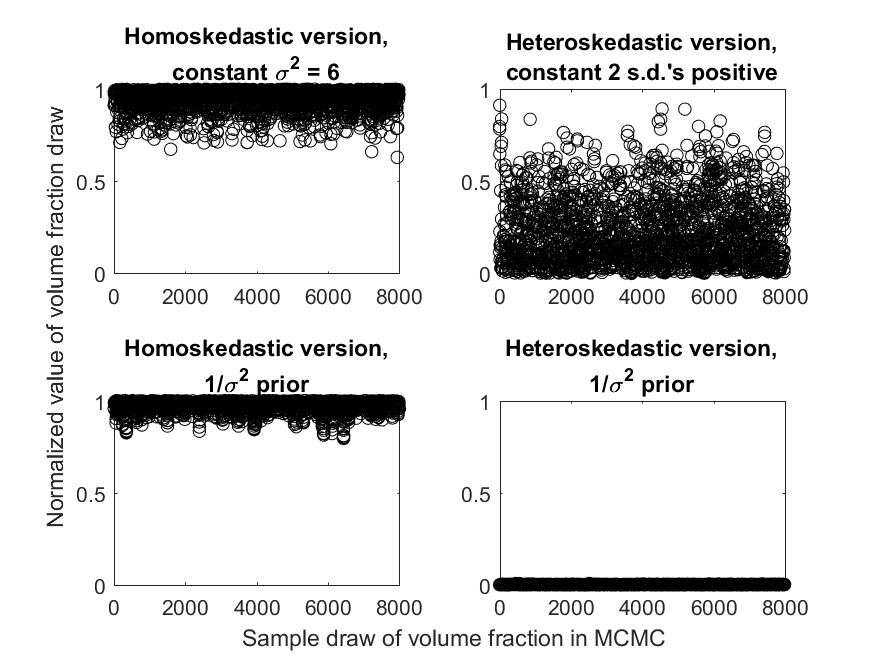
\includegraphics[width=.75\linewidth]{FIG_comp_obs_var}
%\captionsetup{width=.65\linewidth}
%\caption{MCMC results of volume fraction at various observation variance settings, on normalized scale. The heteroskedastic constant variance was chosen so that each of the three desired outputs is two standard deviations above zero; e.g., $\sigma^2_1 = \left(\frac12\cdot 0.65\right)^2\approx0.106$. The homoskedastic constant was set at 6 for each standardized output.}
%\label{fig:comp_obs_var}
%\end{figure}

%% USE scatterhist function -- not sure if this is the right location for it

%\subsection{Which targets to set?}\label{which_data}
%
%A related question to the setting of the observation variance of the desired observation is the setting of the desired observations themselves. I described some general considerations in Section \ref{level_of_desired_data} above, the upshot of which is that it is generally preferable to set desired observations as close to achievable as possible while remaining confident that the observations are not in fact realistically achievable. 
%
%In the case of heteroskedastic observation variance with a (non-degenerate) prior, the specific choice of desired data is not crucial. But where observation variance is either set to a known value or constrained to be equal (up to pre-specified scalar multiple) across outputs, the choice of desired data will matter for the same reason that the constraints on observation variance matter. To see this, consider performing the wind turbine blade calibration with observation variances set equal to $\sigma^2=6$ for all model outputs, where the desired deflection, rotation, and cost are set to $\mathbf d=[0.65,\ 0.077,\ 96]$. These values are the lower bounds on what is known to be plausible ranges for each output. The MCMC results for volume fraction draws and the resulting posterior mean model output for these settings are shown in Figure \ref{fig:comp_obs_var} and Table \ref{table:obs_vvar_comp}. Consider now replacing $\mathbf d$ with $\mathbf d'=[0.65,\ 0.077,\ -500]$. The effect of this would be equivalent to keeping $\mathbf d$ and reducing the observation variance for cost from 6 to a much lower value, insofar as each of these two changes amounts to increasing the Mahalanobis distance of each draw from the desired observation along the axis of cost. This, in turn, would have the effect in the calibration procedure of prioritizing cost at the expense of the performance metrics. Thus when one wishes to strike a balance of priorities in the calibration procedure, this will necessarily involve both constraints upon the observation variance and the choice of desired observations. A further illustration of the impact of this choice is in Table \ref{table:d_comp}, where two different levels of desired observations are compared under a pre-specified constant observation variance.
%
%Figure \ref{fig:des_data} illustrates the sort of difficulty that can arise if one fails to make one's desired observations sufficiently ambitious. Here, a separate $1/\sigma^2_i$ prior was placed on each of the three types of observation variance. The top set of plots show the MCMC results for an appropriately ambitious (i.e. not realistically achievable) desired observations (here rotation has been removed from the model for simplicity). The desired observations yield good mixing in the MCMC routine. In the bottom plots, the desired observation of deflection is still lower than what is realistically achievable, whereas the cost is low but achievable. The model can yield this desired cost, and so draws of the observation variance for cost quickly drift to extremely low values. As a result, the MCMC samples only from the very small region of the parameter space corresponding to cost very near \$163. The extremely strong correlation of VF and thickness within this region can be seen in the bottom right plot of Figure \ref{fig:des_data}. The small size of this region makes it difficult to sample from. But more importantly, samples from this region are not of particular interest, since it is possible to outperform this region in cost without sacrificing other desiderata. If one were antecedently unaware that this region can be outperformed, that fact would be suggested by the ability of the MCMC to find a region that meets the cost target (nearly) exactly without much variation in meeting the other desiderata. Indeed, this outcome of extremely low observation variance -- when observation variance is sampled under a prior -- serves as a way to detect that one's desired observation is in fact realistically achievable.
%
%When one \emph{knowingly} sets a realistically achievable outcome as a desired observation, it is preferable to specify a constant observation variance, or at least a lower bound on observation variance. In this way, one avoids the convergence difficulties of the lower plots in Figure \ref{fig:des_data}. In essence, setting a lower bound on the observation variance of cost would ``fatten'' the thin line of accepted draws represented in the rightmost plot, enhancing the ease with which the MCMC routine can explore the parameter space, and improving the acceptance ratio. However, where an analysis calls for strict adherence to a given target observation (so that such ``fattening'' is unpalatable), tools of low probability estimation can be brought to bear. Sequential Monte Carlo \citep{Doucet2001,Liu2001a} or subset simulation \citep{Au2001a,Au2003,Zuev2012a} can be used to sample from the low-probability space associated with a tight bound on a desired observation.
%%\subsubsection{Differing results}
%% for different desired data values
%\begin{table}[h]
%\centering
%\begin{tabular}{| c | c  | c  |  c | c  | c | c | c |}
%\hline
%Desired data $\mathbf d$ & $\sigma^2_{defl}$ & $\sigma^2_{rot}$ & $\sigma^2_{cost}$ & $\mu_{v|\mathbf d}$ &
%                            $\mu_{h|\mathbf d}$ & $\sigma^2_{v|\mathbf d}$ & $\sigma^2_{h|\mathbf d}$\\
%\hline
%$(0, 0, 0)$ & 375.45 & 277.69 & 2.62 & 0.215 & $4.01 \cdot 10^{-2}$&
%	$4.41\cdot 10^{-2}$ & $1.92 \cdot 10^{-3}$\\
%$(0.65, 0.077, 96)$ & 16.74 & 15.25 & $4.62 \cdot 10^{-7}$ &
%	$1.09 \cdot 10^{-3}$ & $3.36 \cdot10^{-4}$ &
%	$1.02 \cdot 10^{-5}$ & $9.97 \cdot 10^{-6}$\\
%\hline
%\end{tabular}
%\captionsetup{width=.95\linewidth}
%\caption{Comparison of results for two different (low) values of $\mathbf d$. Values listed are, respectively, the posterior means for the observation variance of each model output, posterior means for volume fraction ($v$) and thickness ($h$), and posterior variance of volume fraction and thickness. The differing results reflect different prioritizations of cost over performance metrics, since volume fraction correlates positively with cost and negatively with deflection and rotation.}
%\label{table:d_comp}
%\end{table}
%
%\begin{figure}
%\centering
%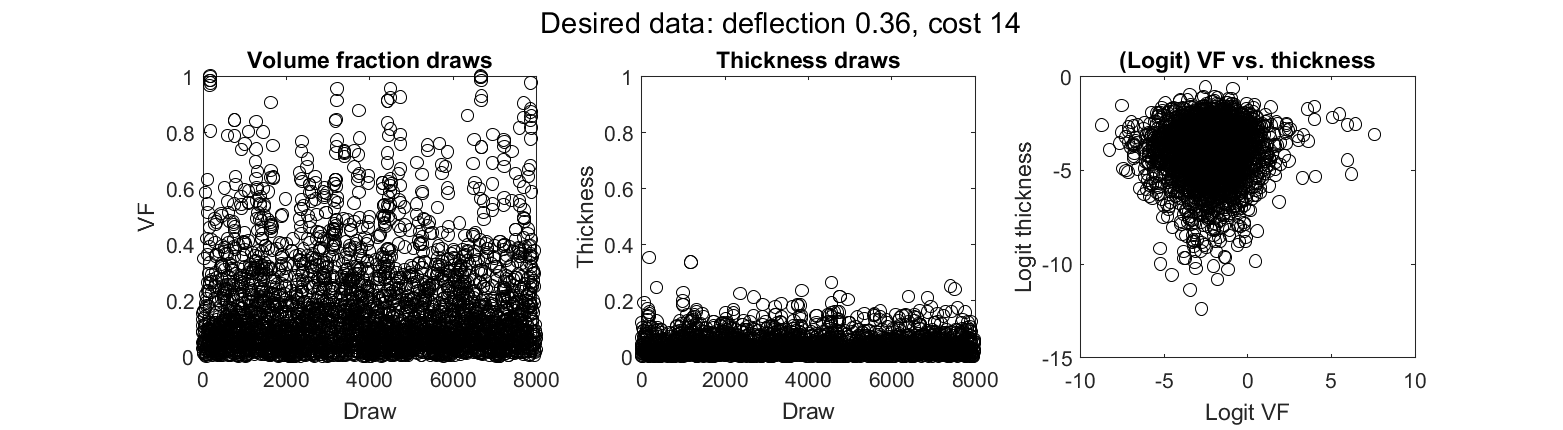
\includegraphics[width=.9\linewidth]{FIG1_posterior_samps_at_spec_cost}
%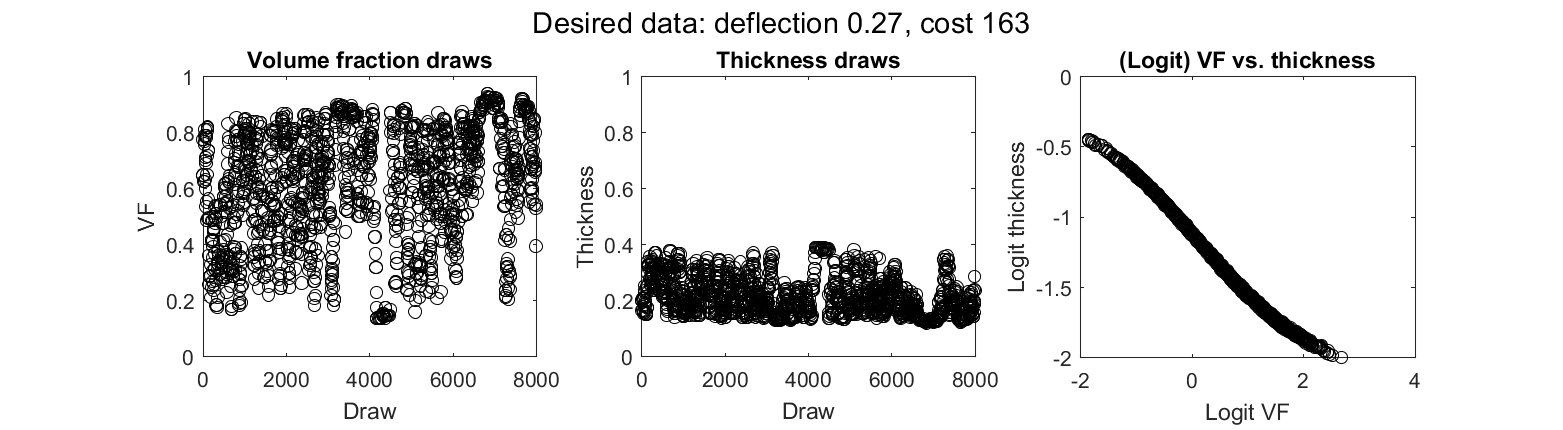
\includegraphics[width=.9\linewidth]{FIG2_posterior_samps_at_spec_cost}
%\captionsetup{width=.9\linewidth}
%\caption{MCMC results for low deflection and cost (top row) and low deflection with easily achievable cost (bottom row).}
%% NOTE: THESE PLOT TITLES ARE WRONG! GOTTA DO THE PLOTS OVER! LOL! but wait are they still
%\label{fig:des_data}
%\end{figure}

%\paragraph{Non-uniform prior on $\boldsymbol \theta$:}\label{non-uniform_prior}
%
%%\subsubsection{Implementation}
%
%The first option is attractive in those scenarios where one has rough knowledge of the correlation between the calibration parameters and a given model output. The strategy is to exploit this correlation to remove one of the desired observation outputs, where a prior is placed on the calibration parameters that is designed to control the removed model output.
%
%The wind turbine application serves as an example here. It is known that cost correlates strongly with each of the two calibration parameters (volume fraction $v$ and thickness $k$). Thus, I replace the uniform $\pi(\boldsymbol \theta)$ of (\ref{eq:the_model}) with a prior that penalizes high values of $v$ and $k$, thereby penalizing high cost output:
%\begin{equation}\label{eq:theta_prior}
%\pi(\boldsymbol \theta)=\pi(v,k)\propto \exp(-\lambda_{cost}\lVert (v,k)\rVert ^2)
%\end{equation}
%where $\lambda_{cost}$ can be set to any nonnegative value, with higher values resulting in stricter cost control. Pairing this with the $1/\sigma^2_i$ prior on observation variances, the full model becomes:
%\begin{equation}\label{full_model_3}
%\begin{aligned}
%\pi(\boldsymbol\theta,\mathbf C_{\mathbf y}|\mathcal D ) &\propto
%\pi(\mathcal D|\boldsymbol\theta,\mathbf C_{\mathbf y}) \times \pi(\boldsymbol\theta) \times \pi(\mathbf C_{\mathbf y})\\
%&\propto \lvert \mathbf C_{\mathcal D} \rvert ^{-1/2} \mathrm{exp}(\mathcal D^T \mathbf C_{\mathcal D}^{-1} \mathcal D) \times \mathrm{exp}(-\lambda_{cost}\lVert(v,k)\rVert^2)\times\prod_{i=1}^3 \frac1{\sigma^2_i}
%\end{aligned}
%\end{equation}
%
%This may seem to make little progress in resolving the complication of a model that includes cost, since now instead of specifying a desired cost we must specify a value for $\lambda_{cost}$. However, rather than specify a value for this hyperparameter, we can gain a more comprehensive picture of our options by observing the calibration results over a grid of values of $\lambda_{cost}$. Thus, rather than specifying beforehand what is our desired ``balance'' amongst cost, deflection and rotation, we are able to see a curve describing our options for this trade-off, and to then make an informed choice as to where on that curve we wish to be. 
%
%The decision-making value of such an analysis is further improved by including uncertainty quantification, which comes easily due to the nature of the Bayesian approach and GP emulator here. The draws of calibration parameters in the MCMC routine each correspond to a GP with posterior mean serving as an estimate of the true model output for those calibration settings. This captures the parameter uncertainty -- i.e., uncertainty remaining in the posterior distribution of the calibration parameters, which is uncertainty about which calibration parameter settings best achieve the desired observations. Furthermore, the GPs themselves are uncertain representations of the true model. For each draw of the calibration parameters in the MCMC routine, (\ref{posterior_GP}) gives us the mean and variance of the output at each control input. Thus we can use the posterior covariance of the GP to estimate the code uncertainty -- the uncertainty due to the variation of the GP around the true system mean. Thus a sort of ``Pareto band'' of model performance can guide decision-making in selecting a level for our calibration parameters. Decision-makers can observe surfaces describing the achievable system responses, with included uncertainty measures around those surfaces, and select a target outcome from this comprehensive picture of what is achievable. Figure \ref{fig:non-uniform_prior} gives an example of this for the wind turbine application. Figure \ref{fig:post_dists_lambda_cost} shows the posterior distributions of volume fraction and thickness for various values of $\lambda_{cost}$. 
%
%\begin{figure}
%\centering
%\captionsetup{width=.9\linewidth}
%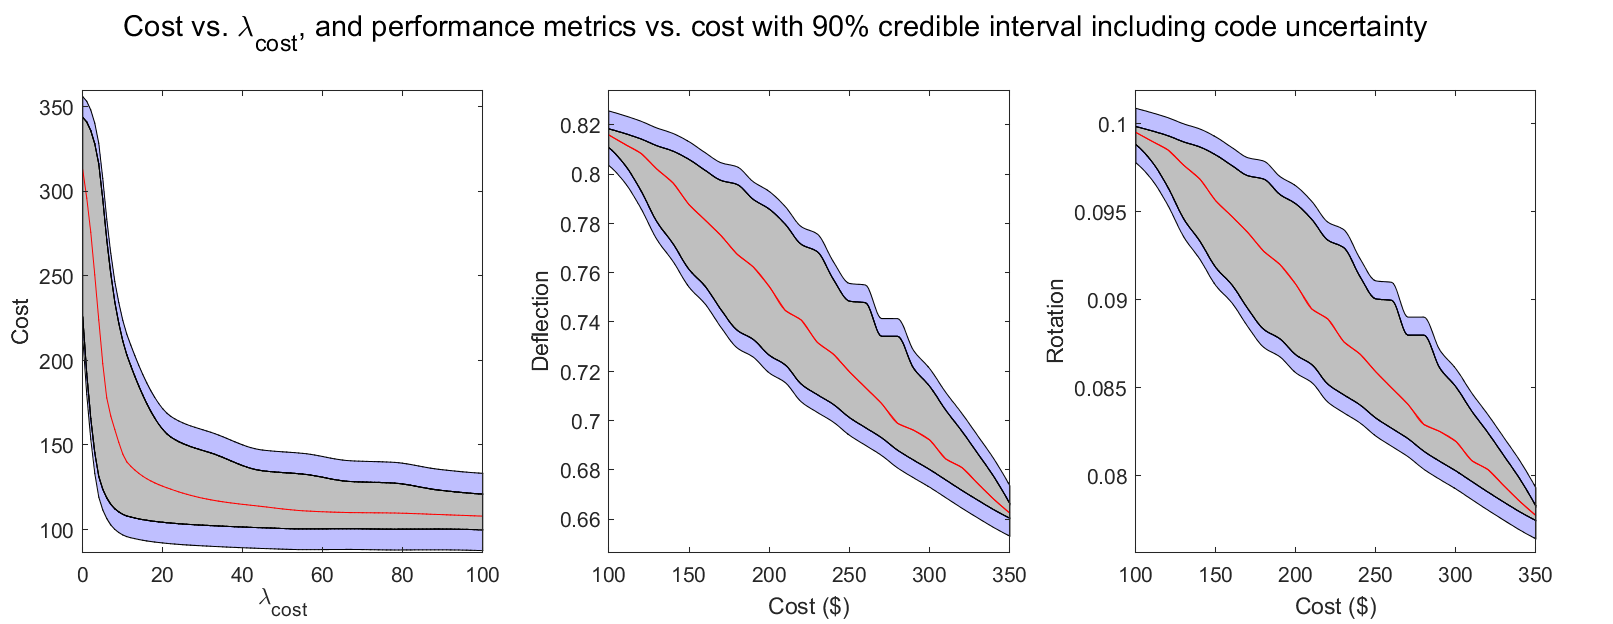
\includegraphics[width=\linewidth]{FIG_cost_lambda_code_uncert_upd}
%\caption{Resulting cost vs. $\lambda_{cost}$, and ``Pareto bands'' of wind turbine blade performance metric over a range of values of cost. Here, cost has been removed from the model and the prior $\exp(-\lambda_{cost}\lVert \theta \rVert^2)$ placed on the calibration parameters $\boldsymbol \theta$, with desired data 0 deflection and 0 rotation. The gray region gives a 90\% credible interval only considering parameter uncertainty. The blue region extends this to include code uncertainty, using the covariance of the posterior GPs corresponding to each draw of $\boldsymbol \theta$.}
%\label{fig:non-uniform_prior}
%\end{figure}
%
%
%\begin{figure}
%\centering
%\captionsetup{width=.7\linewidth}
%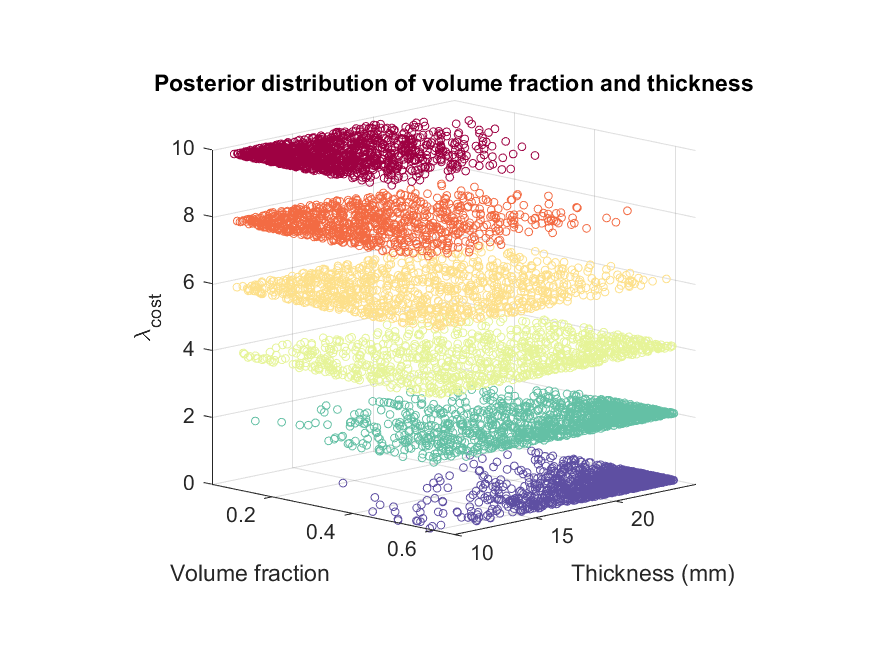
\includegraphics[width=.65\linewidth]{FIG_post_dist_across_cost_lambda-3d}
%\caption{Posterior distributions of volume fraction and thickness for various values of $\lambda_{cost}.$ Notice that higher values of $\lambda_{cost}$ push the distribution away from the (high-cost) upper region of the supports of the two variables.}
%\label{fig:post_dists_lambda_cost}
%\end{figure}

%\subsection{Exponentially distributed desired data}
%Blah

%\subsubsection{Motivation}
%Blah

%\subsubsection{Implementation and results}
%Blah


%\section{Future work}
%
%
%%\subsection{Alternative means of handling cost}
%%Blah
%
%%\subsubsection{Removing cost from the model}
%%Blah
%
%%\subsubsection{Alternative priors for controlling cost}
%%Blah
%
%%\subsection{Building a desired data response surface}
%%Blah
%
%\subsection{Hamiltonian Monte Carlo}
%
%Recall from Figure \ref{ACFs} that the autocorrelation in the MCMC routine, while much reduced by using the Metropolis-Hastings algorithm after applying a logit transformation to remove boundary conditions, is nonetheless still appreciable. In the application considered there, in order to achieve uncorrelated draws, one would save at most every $30^{\text{th} }$ draw. The efficiency of the algorithm can be improved by instead using the Hamiltonian Monte Carlo technique (HMC), also known as hybrid Monte Carlo \citep{Duane1987}. 
%
%Initially applied to lattice field theory simulations of quantum chromodynamics, HMC was popularized within the statistical community by \cite{Neal2011}. Neal describes the intuition supporting HMC roughly as follows. Consider the Metropolis-Hastings algorithm, in which a proposed new draw is drawn from a proposal distribution which is typically centered on the previous draw. Thus the position of the previous draw informs the next proposed draw. Rather than rely merely on the position of the previous draw, HMC relies both on its position and on its \emph{momentum}. The momentum of a variable moving in $p-$dimensional space can be understood on analogy to a puck moving on a horizontal two-dimensional surface curved in the third dimension to have areas of varying height. Negative likelihood for the variable is the analog for height. As the variable moves from an area of low likelihood to higher likelihood, it gains momentum, increasing the proposal density in the direction of that momentum. Likewise, as the variable moves from an area of high likelihood to low likelihood, its momentum can help carry it further into that space; but moving into the low likelihood space also reduces the variable's momentum, eventually causing the momentum to change direction.
%The result of these Hamiltonian dynamics in the sampling routine is to improve the efficiency of the exploration of the parameter space. Thus HMC works to reduce autocorellation beyond what is typically possible in Metropolis-Hastings. Therefore its use in the area of CDO can help to improve the efficiency of the sampling routine beyond what is seen in the righthand panel of Figure \ref{ACFs}.
%
%%\subsubsection{Hamiltonian Monte Carlo}
%% Background
%%Blah
%
%%\subsubsection{Benefits}
%%Blah
%
%\subsection{Model discrepancy}
%
%Recall from Section  \ref{model_shortcoming} that we may incorporate model shortcoming in two ways: as a form of observation variance, or as a form of model discrepancy. In Section \ref{MCMC}, observation variance serves as the basis for handling model shortcoming. This approach is attractive for its simplicity and for its flexibility in facilitating different calibration goals through modulation of the observation variances and their prior distributions. 
%However, as described in Section \ref{mod_disc}, there are advantages to using a model discrepancy $\delta(\cdot)$ instead of observation variance to incorporate model shortcoming. Most importantly, one's desired observation will tend to be systematically biased from the true system mean, and a model that incorporates shortcoming by way of Gaussian white noise, in an observation variance term, fails to capture this systematic bias. For this reason, future work in this area will include replacing observation variance with a prior mean-zero GP discrepancy function in the calibration procedure.
%
%Similarly, the technique of CDO as described in the present work assumes access to a computer model which is known to be accurate throughout the domain $\mathcal T$ over which the calibration occurs. Of course, in many applications, this assumption will not hold. Future extensions of the present work will include investigation of combining CDO with traditional calibration. This would be of interest in those situations where one has access to field observations and wishes to employ CDO. If computational expense makes simulation observations scarce, it will be particularly attractive to combine the two calibrations, using the same set of simulations for both calibrations simultaneously.
%
%I intend to pursue two avenues in this area. Firstly, one might capture model inadequacy with a traditional model discrepancy function, while simultaneously capturing model shortcoming via observation variance. In a full Bayesian analysis that treats desired observations as extra field observations, this would certainly lead to a lack of identifiability between the observation variance and the discrepancy function. However, the method of ``modularization'' \citep{Liu2009,Bayarri2007,Bayarri}, described above in Section \ref{computer_model_calibration}, can mitigate these difficulties, by partitioning the analysis so that desired observations do not bias the discrepancy function, and field observations do not bias the estimate of the observation variance of the desired observations.
%
%Secondly, one may attempt to capture model inadequacy and model shortcoming each in a separate discrepancy function. This will face the same difficulty as the first approach, and will likewise require modularization in order to retain the identifiability of the two discrepancy functions.
%
%\subsection{Comparison with optimization techniques}
%
%CDO is a form of optimization, and thus future work will include a thorough comparison of that approach to alternative forms of optimization. As well as comparing results, computational economy should be considered as a desideratum. Furthermore, CDO is a form of optimization under uncertainty, which can easily incorporate uncertainty in the model inputs, and which delivers a result which includes quantification of uncertainty on the posterior model outputs. Therefore, of particular interest are alternative means of optimization that accommodate and quantify uncertainty. \cite{Sahinidis2004} provides a useful overview of existing techniques for optimization under uncertainty; such techniques are the primary alternatives against which CDO should be considered.
%
%\section{Conclusion}
%% Discussion of the role of computer model validation as a potential methodology for design
%
%In this work I have described the theoretical background for the use of Gaussian processes to emulate computationally expensive computer model code, and the use of such emulators for computer model calibration under the framework established principally by \cite{Kennedy2001}, \cite{Williams2006} and \cite{Bayarri2007}. I have also described a modification of that framework which calibrates a computer model, not to field observations, but rather to desired observations, i.e., performance targets for the system. I described the implementation of this approach in an MCMC routine along with considerations to accommodate computational instability. I have also indicated future directions for research in the area of CDO.
%
%The use of this methodology is illustrated in the case of material design for a wind turbine blade. I have shown thereby a variety of ways in which CDO can be used to produce a guide that decision-makers can consult in the design process. By expropriating established tools of model calibration, CDO offers a method of optimization which is sensitive to all sources of uncertainty, and which results in an estimate that includes uncertainty quantification.
%
%
%\begin{appendices}
%
%\section{Full conditional distributions}
%Using a model that does not employ a discrepancy term, uses maximum likelihood estimation of $\boldsymbol \beta^\eta$ and $\lambda_\eta$, and sets the mean $c$ of the emulator to be 0, we have from \eqref{eq:full_dist} above that the joint posterior distribution is
%\begin{equation}
%\begin{aligned}
%\pi(\boldsymbol\theta,\mathbf C_{\mathbf y} | \mathcal D) &\propto
%\pi(\mathcal D|\boldsymbol\theta,\mathbf C_{\mathbf y}) \times \pi(\boldsymbol\theta) \times \pi(\mathbf C_{\mathbf y})\\
%&\propto \lvert \mathbf C_{\mathcal D} \rvert ^{-1/2} \exp (\mathcal D^T \mathbf C_{\mathcal D}^{-1}\mathcal D) \times \pi(\boldsymbol \theta) \times \pi(\mathbf C_{\mathbf y})
%\end{aligned}
%\end{equation}
%where $\mathbf C_{\mathcal D}$, given in \eqref{eq:C_D}, depends on both $\boldsymbol\theta$ and on $\mathbf C_{\mathbf y}$.
%Different priors on $\boldsymbol\theta$ and $\mathbf C_{\mathbf y}$ are used in the present work to flesh out this distribution. 
%For example, columns one and two of Table \ref{table:obs_vvar_comp} correspond to setting a uniform prior on $\boldsymbol\theta$ and specifying a set value for $\mathbf C_y$ (essentially thereby using a degenerate prior). 
%Thus over the support of $\boldsymbol \theta$ at the specified value of $\mathbf C_{\mathbf y}$, the joint posterior distribution is
%\begin{equation}\label{eq:fdupup}
%\begin{aligned}
%\lvert \mathbf C_{\mathcal D} \rvert ^{-1/2} \exp (\mathcal D^T \mathbf C_{\mathcal D}^{-1}\mathcal D) \times \pi(\boldsymbol \theta) \times \pi(\mathbf C_{\mathbf y}) &=\lvert \mathbf C_{\mathcal D} \rvert ^{-1/2} \exp (\mathcal D^T \mathbf C_{\mathcal D}^{-1}\mathcal D)
%\end{aligned}
%\end{equation}
%and since $\mathbf C_{\mathbf y}$ is specified in advance, this distribution is also the marginal posterior distribution of $\boldsymbol\theta$. 
%By contrast, columns three and four of Table \ref{table:obs_vvar_comp} place a reference prior on the observation variance of each model output. Recall that where $\sigma^2_i$ gives the observation variance for the $i^{th}$ model output, $\mathbf C_{\mathbf y}$ is a diagonal matrix with $i,i$ entry $\sigma^2_i$. 
%Column three of the table corresponds to a model in which each of the three outputs has its own observation variance, so that the prior $\pi(\mathbf C_{\mathbf y})=\prod_{i=1}^3 \sigma^{-2}_i$. 
%Column four uses a single observation variance for all three outputs, so that the prior is $\pi(\mathbf C_{\mathbf y})=\sigma^{-2}$. 
%Letting $K=3$ for column three and $K=1$ for column four, then, the joint posterior distribution is
%\begin{equation}\label{eq:fduprp}
%\begin{aligned}
%\lvert \mathbf C_{\mathcal D} \rvert ^{-1/2} \exp (\mathcal D^T \mathbf C_{\mathcal D}^{-1}\mathcal D) \times \pi(\boldsymbol \theta) \times \pi(\mathbf C_{\mathbf y}) 
%&\propto\lvert \mathbf C_{\mathcal D} \rvert ^{-1/2} \exp (\mathcal D^T \mathbf C_{\mathcal D}^{-1}\mathcal D) \times \prod_{i=1}^K \sigma^{-2}_i
%\end{aligned}
%\end{equation}
%where $\pi(\boldsymbol\theta)$ is again set to be uniform.
%Thus the posterior conditional distributions are
%\begin{equation}\label{eq:cduprp}
%\begin{aligned}
%\pi(\boldsymbol\theta|\mathbf C_{\mathbf y},\mathcal D) &\propto
%\lvert \mathbf C_{\mathcal D} \rvert ^{-1/2} \exp (\mathcal D^T \mathbf C_{\mathcal D}^{-1}\mathcal D) \\
%\pi(\mathbf C_{\mathbf y}| \boldsymbol \theta ,\mathcal D) &\propto
%\lvert \mathbf C_{\mathcal D} \rvert ^{-1/2} \exp (\mathcal D^T \mathbf C_{\mathcal D}^{-1}\mathcal D) \times \prod_{i=1}^K \sigma^{-2}_i.
%\end{aligned}
%\end{equation}
%
%Section \ref{removing_cal_pars} employs a model which places an informative prior on $\boldsymbol \theta$. A reference prior is also placed on the observation variance of each model output. The resulting posterior distribution is thus
%\begin{equation}\label{eq:fdifrp}
%\begin{aligned}
%\lvert \mathbf C_{\mathcal D} \rvert ^{-1/2} \exp (\mathcal D^T \mathbf C_{\mathcal D}^{-1}\mathcal D) \times \pi(\boldsymbol \theta) \times \pi(\mathbf C_{\mathbf y}) 
%&\propto\lvert \mathbf C_{\mathcal D} \rvert ^{-1/2} \exp (\mathcal D^T \mathbf C_{\mathcal D}^{-1}\mathcal D) \times 
%\exp(-\lambda_{cost} \lVert \boldsymbol\theta\rVert^2) \times
%\prod_{i=1}^3 \sigma^{-2}_i
%\end{aligned}
%\end{equation}
%and the posterior conditional distributions are given by
%\begin{equation}\label{eq:cdifrp}
%\begin{aligned}
%\pi(\boldsymbol\theta|\mathbf C_{\mathbf y},\mathcal D) 
%&\propto \lvert \mathbf C_{\mathcal D} \rvert ^{-1/2} \exp (\mathcal D^T \mathbf C_{\mathcal D}^{-1}\mathcal D) \times 
%\exp(-\lambda_{cost} \lVert \boldsymbol\theta\rVert^2)\\
%\pi(\mathbf C_{\mathbf y}| \boldsymbol \theta ,\mathcal D) &\propto
%\lvert \mathbf C_{\mathcal D} \rvert ^{-1/2} \exp (\mathcal D^T \mathbf C_{\mathcal D}^{-1}\mathcal D) \times 
%\prod_{i=1}^3 \sigma^{-2}_i.
%\end{aligned}
%\end{equation}
%%Notice that this model includes the model of \eqref{eq:fduprp} and \eqref{eq:cduprp} as a special case, by setting $\lambda_{cost}=0$.
%
%\section{Algorithm for MCMC}
%
%The following algorithm describes how to sample from the model given in \eqref{eq:fdifrp} and \eqref{eq:cdifrp}, which includes the model of \eqref{eq:fduprp} and \eqref{eq:cduprp} as a special case, by setting $\lambda_{cost}=0$. 
%Minor and straightforward modifications are required to sample from the model of \eqref{eq:fdupup}. In the algorithm, single-variable functions applied to multivariate input are applied componentwise; e.g., $\exp\left(\mathrm MVN([0, 0]^T,I_2)\right)$ denotes $[\exp(r_1), \exp(r_2)]$ where $[r_1, r_2]^T\sim\mathrm{MVN}([0, 0]^T,I_2)$.
%
%\begin{algorithm}
%%    \SetKwInOut{Input}{Input}
%%    \SetKwInOut{Output}{Output}
%%
%%    \underline{function Euclid} $(a,b)$\;
%%    \Input{Two nonnegative integers $a$ and $b$}
%%    \Output{$\gcd(a,b)$}
%%    \eIf{$b=0$}
%%      {
%%        return $a$\;
%%      }
%%      {
%%        return Euclid$(b,a\mod b)$\;
%%      }
%\textbf{Step 1:} Draw $\boldsymbol \theta^{(0)}\sim \mathrm {Unif}([0,1]^2)$, $(\sigma^2_j)^{(0)} \sim \mathrm {Gamma}(2,2)$ for $j=1,2,\ldots,K$. 
%Set $\mathbf C_{\mathbf y}$ using $(\sigma^2_j)^{(0)},\ j=1,2,\ldots,K$.
%Set $\mathbf C_{\mathcal D}$ using $\boldsymbol\theta^{(0)}$ and $\mathbf C_{\mathbf y}$.
%Specify $s^2=1$. 
%Specify $\lambda_{cost}\geq0$. Specify total number of iterations $M$ and burn-in $b$.
%Set $\mathrm{mult}=2$.
%Set $\Sigma=I_2$.
%Set $A=0$ and $A_\sigma=0$.
%Set $i=0$.
%
%\textbf{Step 2:} Repeat $M$ times.
%\begin{itemize}
%\item Update $i = i+1$.
%\item Draw $\boldsymbol \theta ^* \sim \mathrm{logit}^{-1}\left( \mathrm{MVN}(\mathrm{logit}(\boldsymbol \theta^{(i-1)}),\Sigma)\right)$.
%\item Set $\mathbf C_{\mathcal D}^*$ using $\boldsymbol\theta^*$ and $\mathbf C_{\mathbf y}$.
%\item Find 
%\begin{align*}
%\log \alpha = &
%\log \left( \lvert \mathbf C^*_{\mathcal D}\rvert^{-1/2} \exp(\mathcal D^T \mathbf {C_{\mathcal D}^*}^{-1}\mathcal D) \right) - 
%\lambda_{cost} \cdot \lVert \boldsymbol\theta^*\rVert^2 - 
%\log \left( \lvert \mathbf C_{\mathcal D}\rvert^{-1/2} \exp(\mathcal D^T \mathbf C_{\mathcal D}^{-1}\mathcal D) \right)  \\&+
%\lambda_{cost} \cdot \lVert \boldsymbol\theta^{(i-1)}\rVert^2 +
%\log \left ( \prod_{j=1}^2 \left( \theta^*_j(1-\theta_j^*) \right) \right ) - 
%\log \left (  \prod_{j=1}^2 \left( \theta^{(i-1)}_j(1-\theta_j^{(i-1)}) \right) \right )
%\end{align*}
%\item Draw $a\sim \mathrm{Unif}(0,1)$. If $a<\alpha$, set $\boldsymbol\theta^{(i)}=\boldsymbol\theta^*$, $\mathbf C_{\mathcal D} = \mathbf C_{\mathcal D}^*$, and increment $A=A+1$; otherwise, set $\boldsymbol\theta^{(i)} = \boldsymbol\theta^{(i-1)}$.
%\item Draw $[{\sigma_1^2}^*, {\sigma_2^2}^*, {\sigma_3^2}^*]^T \sim \exp \left ( \mathrm {MVN}\left( \log\left[{\sigma_1^2}^{(i-1)}, {\sigma_2^2}^{(i-1)}, {\sigma_3^2}^{(i-1)} \right]^T, s^2I_3 \right) \right)$.
%%\item Find $\log \alpha = \log \left( \lvert \mathbf C^*_{\mathcal D}\rvert^{-1/2} \exp(\mathcal D^T \mathbf {C_{\mathcal D}^*}^{-1}\mathcal D) \right) - \log\left(\prod_{j=1}^K {\sigma^2_k}^* \right)
%%- \log \left( \lvert \mathbf C_{\mathcal D}\rvert^{-1/2} \exp(\mathcal D^T \mathbf C_{\mathcal D}^{-1}\mathcal D) \right) + \log\left(\prod_{j=1}^K {\sigma^2_k}^{(i-1)} \right)
%%+ \log \left ( \prod_{j=1}^2 \left( \theta^*_j(1-\theta_j^*) \right) \right ) - \log \left (  \prod_{j=1}^2 \left( \theta^{(i-1)}_j(1-\theta_j^{(i-1)}) \right) \right )$.
%%\item Draw $\left[{\sigma^2_1}^*,{\sigma^2_2}^*,{\sigma^2_3}^*\right]^T\sim\exp\left ( \mathrm {MVN} \left ( \log \left[{\sigma^2_1}^{(i-1)},{\sigma^2_2}^{(i-1)},{\sigma^2_3}^{(i-1)}\right]^T,s^2I_3\right)\right) $
%\item Set $\mathbf C_{\mathbf y}^*$ using $\left[{\sigma^2_1}^*,{\sigma^2_2}^*,{\sigma^2_3}^*\right]^T$. Set $\mathbf C_{\mathcal D}^*$ using $\boldsymbol \theta^{(i)}$ and $\mathbf C_{\mathbf y}^*$.
%\item Find $\log \alpha = \log \left( \lvert \mathbf C^*_{\mathcal D}\rvert^{-1/2} \exp(\mathcal D^T \mathbf {C_{\mathcal D}^*}^{-1}\mathcal D) \right) - \log \left( \lvert \mathbf C_{\mathcal D}\rvert^{-1/2} \exp(\mathcal D^T \mathbf C_{\mathcal D}^{-1}\mathcal D) \right)$. 
%(Notice that the log ratio of priors $\log \left( \frac{\pi({\sigma^2_i}')}{\pi(\sigma^2_i)}\right)=\log \frac{{\sigma^2_i}}{{\sigma^2_i}'} = \log{\sigma^2_i}-\log{\sigma^2_i}'$ is cancelled out by the log Metropolis-Hastings correction for the asymetrical proposal density: $\log \left ( \frac{q(\sigma^2_i|{\sigma^2_i}')}{q({\sigma^2_i}'|\sigma^2_i)} \right)= \log\left( \frac{{\sigma^2_i}'}{\sigma^2_i} \right)= \log {\sigma^2_i}'- \log \sigma^2_i $.)
%\item Draw $a\sim \mathrm{Unif}(0,1)$. If $a<\alpha$, set $\left[{\sigma_1^2}^{(i)}, {\sigma_2^2}^{(i)}, {\sigma_3^2}^{(i)} \right]^T = \left[{\sigma_1^2}^{*}, {\sigma_2^2}^{*}, {\sigma_3^2}^{*} \right]^T$, $\mathbf C_{\mathbf y} = \mathbf C_{\mathbf y}^*$, $\mathbf C_{\mathcal D} = \mathbf C_{\mathcal D}^*$, and increment $A_\sigma = A_\sigma + 1$; otherwise, set $\left[{\sigma_1^2}^{(i)}, {\sigma_2^2}^{(i)}, {\sigma_3^2}^{(i)} \right]^T = \left[{\sigma_1^2}^{(i-1)}, {\sigma_2^2}^{(i-1)}, {\sigma_3^2}^{(i-1)} \right]^T$.
%\item If $i\leq b$ and $i\pmod {100} = 0$:
%\renewcommand{\labelitemii}{$\circ$}
%\begin{itemize}
%\item Update $\mathrm {mult} = 1.5 \cdot \mathrm{mult} \cdot \mathbf 1_{A>30} + 0.75 \cdot \mathrm {mult} \cdot \mathbf 1_{A<20}$. Set $A=0$.
%\item Update $\Sigma= \mathrm{mult} \cdot \mathrm {Cov}\left(\Theta\right)$, where $\Theta=\left[ {\boldsymbol\theta^{(1)}}, {\boldsymbol\theta^{(2)}}, \ldots, {\boldsymbol\theta^{(i)}} \right]^T$.
%\item Update $s^2 = 1.5 \cdot s^2 \cdot \mathbf 1_{A_\sigma>30} + 0.75 \cdot s^2 \cdot \mathbf 1_{A_\sigma<20}$. Set $A_\sigma=0$.
%\end{itemize}
%\end{itemize}
%    \caption{}
%\end{algorithm}
%
%
%
%
%\end{appendices}

